%
% Honours Thesis template that uses the memoir package
%
\documentclass[a4paper,12pt,openany]{memoir}

% \usepackage{lmodern}
% \usepackage[T1]{fontenc}

\usepackage{titlesec}

\usepackage{setspace}
\linespread{1.5}

\usepackage{amsmath,amssymb,amsthm}
\usepackage{graphicx,color,xcolor}
\usepackage{thmtools}
\usepackage[linktocpage=true]{hyperref}


\usepackage{tikz}
\usetikzlibrary{calc,backgrounds}
\usepackage{amsmath}
\usepackage{amssymb}
\usepackage{float}
\usepackage{graphicx}
\usepackage{svg}
\usepackage{pgfplots}
\usepackage[table]{xcolor}
\usepackage{subcaption}

% turn off blank pages for double-page clears
\let\origcleardoublepage\cleardoublepage
\let\cleardoublepage\clearpage

\setcounter{MaxMatrixCols}{20} % Increase max allowed columns

\usetikzlibrary{fadings}
\tikzfading
  [name=fadeLR,
   left color=transparent!100,  % fully transparent at the left
   right color=transparent!0]   % fully opaque at the right
\tikzfading
   [name=fadeRL,
    right color=transparent!100,  % fully transparent at the left
    left color=transparent!0]   % fully opaque at the right

\definecolor{pale_yellow}{HTML}{ffef96}

\definecolor{col1}{HTML}{7570B3}
\definecolor{col2}{HTML}{D95F02}
\definecolor{col3}{HTML}{1B9E77}
\definecolor{col4}{HTML}{E7298A}
\definecolor{col5}{HTML}{66A61E}
\definecolor{col6}{HTML}{E6AB02}

\definecolor{col1_light}{HTML}{8f8ac0}
\definecolor{col2_light}{HTML}{d88a5f}
\definecolor{col3_light}{HTML}{6fb89f}
\definecolor{col4_light}{HTML}{e08fb5}
\definecolor{col5_light}{HTML}{8fb87f}
\definecolor{col6_light}{HTML}{e0c15a}



\hypersetup{
    colorlinks,
    linkcolor={blue!90!black},
    citecolor={blue!90!black},
    urlcolor={blue!90!black}
}

\newtheorem{theorem}{Theorem}[section] 
\newtheorem{lemma}[theorem]{Lemma}    
\newtheorem{propn}[theorem]{Proposition}    
\newtheorem{corollary}[theorem]{Corollary}    
\newtheorem{example}[theorem]{Example}    
\newtheorem{question}[theorem]{Question}    
\newtheorem{exercise}[theorem]{Exercise}    
\newtheorem{conjecture}[theorem]{Conjecture}
\newtheorem{definition}[theorem]{Definition}
\newtheorem{property}[theorem]{Property}
\newtheorem{claim}{Claim}
\newtheorem{fact}{Fact}
\newtheorem{remark}[theorem]{Remark}
\newtheorem{problem}[theorem]{Problem}


\declaretheoremstyle[
  headfont=\normalfont\bfseries,
  numbered=unless unique,
  bodyfont=\normalfont,
  spaceabove=1em plus 0.75em minus 0.25em,
  spacebelow=1em plus 0.75em minus 0.25em,
  qed=$\bullet$,
]{exmpstyle2}

\declaretheorem[
  style=exmpstyle2,
  title=Example,
  refname={example,examples},
  Refname={Example,Examples}
]{example2}

\renewcommand{\le}{\leqslant}
\renewcommand{\ge}{\geqslant}
\renewcommand{\leq}{\leqslant}
\renewcommand{\geq}{\geqslant}

% \setlrmarginsandblock{4cm}{2cm}{*}
\setlrmarginsandblock{2.5cm}{2.5cm}{*}
\setulmarginsandblock{2.5cm}{2.5cm}{*}
\checkandfixthelayout








%── define chapter style ──────────────────────────────────────────────────────
% \titleformat{\chapter}[display]
%   {\normalfont\Huge\bfseries\filcenter}         % base format (for title)
%   {\normalfont\LARGE Chapter \thechapter}       % ← label in smaller font
%   {1ex}                                         % separation
%   {\Huge}                                       % title itself in \Huge
%   [\vspace{1ex}\titlerule]                      % rule after
%   \titlespacing*{\chapter}{0pt}{-1em}{20pt}       
%──────────────────────────────────────────────────────────────────────────────


%── define configurable chapter prefix label ─────────────────────────────────
\newcommand{\chapterlabel}{Appendix}% default label; override with \renewcommand{\chapterlabel}{...}
\titleformat{\chapter}[display]
  {\normalfont\Huge\bfseries\filcenter}         % base format (for title)
  {\normalfont\LARGE\chapterlabel\ \thechapter}% use macro for label
  {1ex}                                         % separation
  {\Huge}                                       % title itself in \Huge
  [\vspace{1ex}\titlerule]                      % rule after
\titlespacing*{\chapter}{0pt}{-1em}{20pt}       
%──────────────────────────────────────────────────────────────────────────────









% \chapterstyle{bringhurst}   % you can easily change the chapter style here
\nouppercaseheads
\tightlists

\graphicspath{ {Images/} }

\makeindex

\begin{document}

\begin{titlingpage}

\vspace*{0.4cm}
\begin{center}
{ \huge \bfseries Feature Selection of Ordinal Partitions for Echo State Networks  \\[0.4cm] }
\vspace{1cm}
\end{center}
\begin{center}
\large
by\\
\vspace{1.5cm}
\textbf{Hector Morlet}\\
BSc\\
\vspace{1cm}
\end{center}
\vspace{3cm}

\begin{tabular}{ p{2.2cm}l } 
Supervisors: & Professor Michael Small\\
			&  Doctor Eugene Tan
\end{tabular}

\vfill
\begin{center}
This thesis is presented for the partial requirements of the degree of\\ Bachelor of Science with honours
of the University of Western Australia.\\
\today
\end{center}
\vspace{2.5cm}
\end{titlingpage}

\frontmatter
\chapter*{Abstract}
\addcontentsline{toc}{chapter}{Abstract}

This thesis will present research into the use of the ordinal partitioning of time series data to inform the creation of an Echo State Network to predict this data.
\chapter*{Acknowledgements}
\addcontentsline{toc}{chapter}{Acknowledgements}

This thesis is the result of the many patient meetings and helpful guidance provided by Eugene and Michael, and I am very grateful for their support.

\tableofcontents
\newpage
\listoffigures 
\newpage
\listoftables

\mainmatter
% !TEX root = ../HonoursThesisTemplate.tex

\chapter{Echo State Networks}


    \begin{itemize}
        \item First introduced by Jaeger (2001). %TODO reference
        \item Type of recurrent neural network.
        \item Commonly studied form of reservoir computing.
        \item A form of supervised learning.
        \item Most weights are fixed and only some are fitted.
        \item Is computationally efficient compared to other neural networks.
    \end{itemize}

    








    State update equation:
    \[
        \mathbf{s}(t + 1) = f_{act}(\mathbf{W}_{in}x(t) + \mathbf{W}_{rec}\mathbf{s}(t) + \mathbf{W}_{bias})
    \]
    \begin{itemize}
        % \begin{itemize}
        %     \item Given a sufficiently long input sequence, the current state of the reservoir is determined uniquely by the intervening input and is independent of its initial state.
        % \end{itemize} % TODO reference here
        \item $\mathbf{W}_{in}$, $\mathbf{W}_{rec}$, $\mathbf{W}_{bias}$ and $\mathbf{s}(t)$ are randomly generated according to hyper-parameters.
        % \item $\mathbf{W}_{rec}$ is a randomly generated network weight matrix (e.g. Erdos-Renyi).
        \item Echo state property
        \item $\mathbf{W}_{in}$, $\mathbf{W}_{rec}$ and $\mathbf{W}_{bias}$ are fixed.
        \item Only the readout vector weights is fitted. % TODO reference A practical guide to applying echo state networks
    \end{itemize}

    









    Output equation:
    \[
        y(t) = \mathbf{C}_{out}\mathbf{s}(t)
    \]
    \[
        \mathbf{Y} = \mathbf{C}_{out}\mathbf{S}
    \]

    Output regression with regularisation: % TODO reference [4] in Lucas'
    \[
        \mathbf{C}_{out} = (\mathbf{S}^T \mathbf{S} + \beta \mathbf{I}) \ \mathbf{S}^T \mathbf{Y}
    \]

    \begin{figure}
        
    %     \centering
        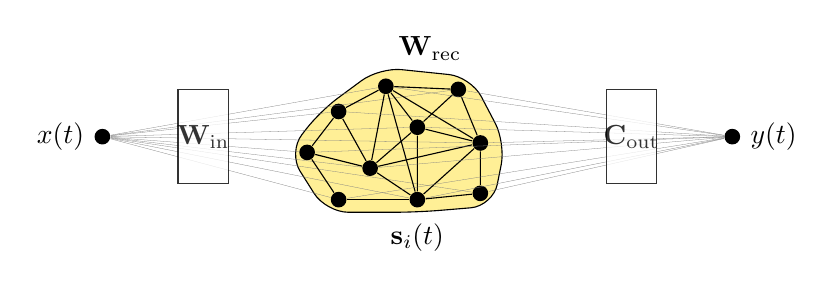
\begin{tikzpicture}[scale=0.8]
            \node[fill=black,circle,inner sep=2pt,label=left:$x(t)$] (input) at (0,0) {};
            \node[fill=black,circle,inner sep=2pt,label=right:$y(t)$] (output) at (10,0) {};
            
            
            \coordinate (res_anchor) at (2,3);
            \node[fill=black,circle,inner sep=2pt] (res1) at ({5-0.5},{0.8}) {};
            \node[fill=black,circle,inner sep=2pt] (res2) at ({5},{-1}) {};
            \node[fill=black,circle,inner sep=2pt] (res3) at ({5},{0.15}) {};
            \node[fill=black,circle,inner sep=2pt] (res4) at ({5+1},{-0.1}) {};
            \node[fill=black,circle,inner sep=2pt] (res5) at ({5-0.75},{-0.5}) {};
            \node[fill=black,circle,inner sep=2pt] (res6) at ({5-1.25},{0.4}) {};
            \node[fill=black,circle,inner sep=2pt] (res7) at ({5+0.65},{0.75}) {};
            \node[fill=black,circle,inner sep=2pt] (res8) at ({5+1},{-0.9}) {};
            \node[fill=black,circle,inner sep=2pt] (res9) at ({5-1.25},{-1}) {};
            \node[fill=black,circle,inner sep=2pt] (res10) at ({5-1.75},{-0.25}) {};
        
            \foreach \i in {1,...,10}
                \draw[gray,line width=0.1] (input) -- (res\i);
            
            \foreach \i in {1,...,5}
                \foreach \j in {1,...,5} {
                    \ifnum\i<\j
                        \draw (res\i) -- (res\j);
                    \fi
                }
            
            \draw (res6) -- (res5);
            \draw (res6) -- (res1);
            \draw (res6) -- (res10);
            \draw (res10) -- (res5);
            \draw (res9) -- (res10);
            \draw (res9) -- (res2);
            \draw (res7) -- (res1);
            \draw (res7) -- (res3);
            \draw (res7) -- (res4);
            \draw (res8) -- (res4);
            \draw (res8) -- (res2);
            
            \foreach \i in {1,...,10}
                \draw[gray,line width=0.1] (res\i) -- (output);
            
            \begin{scope}[on background layer]
            \draw[draw=black,fill=pale_yellow,rounded corners=8pt]  ($(res1)+(-0.1,0.3)$) -- ($(res7)+(+0.2,+0.2)$) -- ($(res4)+(0.4,0)$) -- ($(res8)+(0.2,-0.2)$) -- ($(res2)+(0,-0.2)$) -- ($(res9)+(-0.2,-0.2)$) -- ($(res10)+(-0.3,0)$) -- ($(res6)+(-0.3,0)$) -- cycle;
            \end{scope}
            \node at (5.2, 1.4) {$\mathbf{W}_{\text{rec}}$};
            \node at (5, -1.6) {$\mathbf{s}_i(t)$};
            
            \draw[fill=white,opacity=0.8] (1.2,-0.75) rectangle (2.0,0.75) node[midway] {$\mathbf{W}_{\text{in}}$};
            \draw[fill=white,opacity=0.8] (8, -0.75) rectangle (8.8,0.75) node[midway] {$\mathbf{C}_{\text{out}}$};
        \end{tikzpicture}
        \caption{A diagram of an Echo State Network.}
        \label{fig:ESN}
    \end{figure}

    







% !TEX root = ../HonoursThesisTemplate.tex

\chapter{Ordinal Partitions}

    
`Ordinal analysis', first introduced by Bandt and Pompe (2002), proposed using the ordering of data points to partition a time series. Each data point in the timeseries is partitioned according to the ordering of its preceding points, and assigned a unique `ordinal symbol', for example numbers from 1 to 6.

The probabilities of the timeseries transitioning from one partition to another can be calculated, giving the `ordinal transition probabilities'.

\begin{figure}
    \centering
    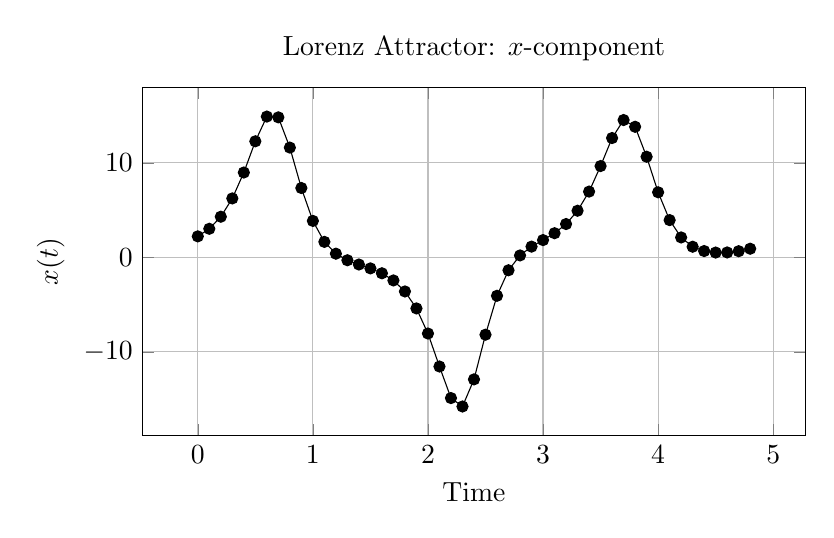
\begin{tikzpicture}
        \begin{axis}[
            xlabel={Time},
            ylabel={$x(t)$},
            title={Lorenz Attractor: $x$-component},
            width=10cm, height=6cm,
            grid=major
        ]
        % Data generated by solving dx/dt = sigma(y - x), etc. in Python
        \addplot[black, mark=*, mark options={black}] coordinates {
            (0.0, 2.2165566502619796)
            (0.1, 3.0181360987381685)
            (0.2, 4.2948078524935065)
            (0.3, 6.231121537780632)
            (0.4, 8.970926893912857)
            (0.5, 12.272230400810887)
            (0.6, 14.887997312478161)
            (0.7, 14.803117347063516)
            (0.8, 11.606868473299526)
            (0.9, 7.330990437181266)
            (1.0, 3.85191889651296)
            (1.1, 1.6347534154776406)
            (1.2, 0.3853895148599277)
            (1.3, -0.30838099414996695)
            (1.4, -0.7586726217449103)
            (1.5, -1.1695821908357407)
            (1.6, -1.6858338981790886)
            (1.7, -2.443141458426554)
            (1.8, -3.6086854451117074)
            (1.9, -5.40339197322587)
            (2.0, -8.058505977971057)
            (2.1, -11.547145254692042)
            (2.2, -14.884182443761347)
            (2.3, -15.775516623377253)
            (2.4, -12.908181797239536)
            (2.5, -8.181376578133673)
            (2.6, -4.06724026097539)
            (2.7, -1.3665393788429014)
            (2.8, 0.20110496364168012)
            (2.9, 1.1324784341364973)
            (3.0, 1.8245674314417792)
            (3.1, 2.5516132966355554)
            (3.2, 3.5214281335608555)
            (3.3, 4.926987945369609)
            (3.4, 6.951562500713474)
            (3.5, 9.654345729238477)
            (3.6, 12.617195234374243)
            (3.7, 14.521825487882024)
            (3.8, 13.806356286601272)
            (3.9, 10.64113968132102)
            (4.0, 6.880279139891668)
            (4.1, 3.9367704788159394)
            (4.2, 2.1029851064946445)
            (4.3, 1.121305395878461)
            (4.4, 0.665491176850325)
            (4.5, 0.5051437108082056)
            (4.6, 0.5156168027361644)
            (4.7, 0.6490783162490397)
            (4.8, 0.9105168761220792)
        };
        \end{axis}
    \end{tikzpicture}
    \caption{This is the caption}
    \label{fig:label}
\end{figure}

\begin{figure}
    \begin{center}
        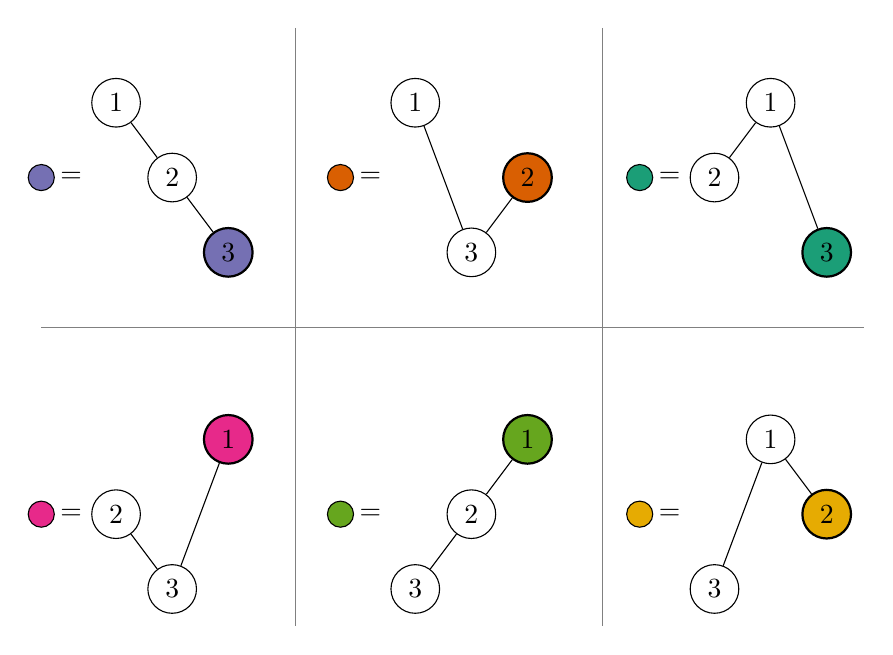
\begin{tikzpicture}[scale=0.95]
            % partition 1

            \node[circle, draw, fill=col1] (topleft) at (-5.0, 3) {};

            % Draw the equality sign
            \node at (-4.6, 3) {$=$};
            
            % Draw the nodes in the lower part
            \node[circle, draw] (1_2) at (-4.0, 4) {1};
            \node[circle, draw] (1_1) at (-3.25, 3) {2};
            \node[circle, draw, thick, fill=col1] (1_3) at (-2.5, 2) {3};
            
            % Draw edges
            \draw (1_1) -- (1_2);
            \draw (1_1) -- (1_3);

            % Draw dividing line
            \draw[gray, very thin] (-1.6, 5) -- (-1.6, -3);

            % partition 2

            \node[circle, draw, fill=col2] (topcentre) at (-1, 3) {};

            % Draw the equality sign
            \node at (-0.6, 3) {$=$};
            
            % Draw the nodes in the lower part
            \node[circle, draw] (2_2) at (0, 4) {1};
            \node[circle, draw] (2_1) at (0.75, 2) {3};
            \node[circle, draw, thick, fill=col2] (2_3) at (1.5, 3) {2};
            
            % Draw edges
            \draw (2_1) -- (2_2);
            \draw (2_1) -- (2_3);

            % Draw dividing line
            \draw[gray, very thin] (2.5, 5) -- (2.5, -3);

            % partition 3

            \node[circle, draw, fill=col3] (topleft) at (3.0, 3) {};

            % Draw the equality sign
            \node at (3.4, 3) {$=$};
            
            % Draw the nodes in the lower part
            \node[circle, draw] (3_2) at (4.0, 3) {2};
            \node[circle, draw] (3_1) at (4.75, 4) {1};
            \node[circle, draw, thick, fill=col3] (3_3) at (5.5, 2) {3};
            
            % Draw edges
            \draw (3_1) -- (3_2);
            \draw (3_1) -- (3_3);

            % Draw dividing line
            \draw[gray, very thin] (-5, 1) -- (6, 1);

            % partition 4

            \node[circle, draw, fill=col4] (bottomleft) at (-5.0, -1.5) {};

            % Draw the equality sign
            \node at (-4.6, -1.5) {$=$};
            
            % Draw the nodes in the lower part
            \node[circle, draw] (4_2) at (-4.0, -1.5) {2};
            \node[circle, draw] (4_1) at (-3.25, -2.5) {3};
            \node[circle, draw, thick, fill=col4] (4_3) at (-2.5, -0.5) {1};
            
            % Draw edges
            \draw (4_1) -- (4_2);
            \draw (4_1) -- (4_3);

            % Draw dividing line
            % \draw[gray, very thin] (-2.25, -3) -- (-2.25, -5);

            % partition 5

            \node[circle, draw, fill=col5] (bottomcentre) at (-1, -1.5) {};

            % Draw the equality sign
            \node at (-0.6, -1.5) {$=$};
            
            % Draw the nodes in the lower part
            \node[circle, draw] (5_2) at (0, -2.5) {3};
            \node[circle, draw] (5_1) at (0.75, -1.5) {2};
            \node[circle, draw, thick, fill=col5] (5_3) at (1.5, -0.5) {1};
            
            % Draw edges
            \draw (5_1) -- (5_2);
            \draw (5_1) -- (5_3);

            % partition 6

            \node[circle, draw, fill=col6] (bottomright) at (3.0, -1.5) {};

            % Draw the equality sign
            \node at (3.4, -1.5) {$=$};
            
            % Draw the nodes in the lower part
            \node[circle, draw] (6_2) at (4.0, -2.5) {3};
            \node[circle, draw] (6_1) at (4.75, -0.5) {1};
            \node[circle, draw, thick, fill=col6] (6_3) at (5.5, -1.5) {2};
            
            % Draw edges
            \draw (6_1) -- (6_2);
            \draw (6_1) -- (6_3);
        \end{tikzpicture}
    \end{center}
    \caption{this is the caption}
    \label{fig:labelhere}
\end{figure}

\begin{figure}
    \centering
    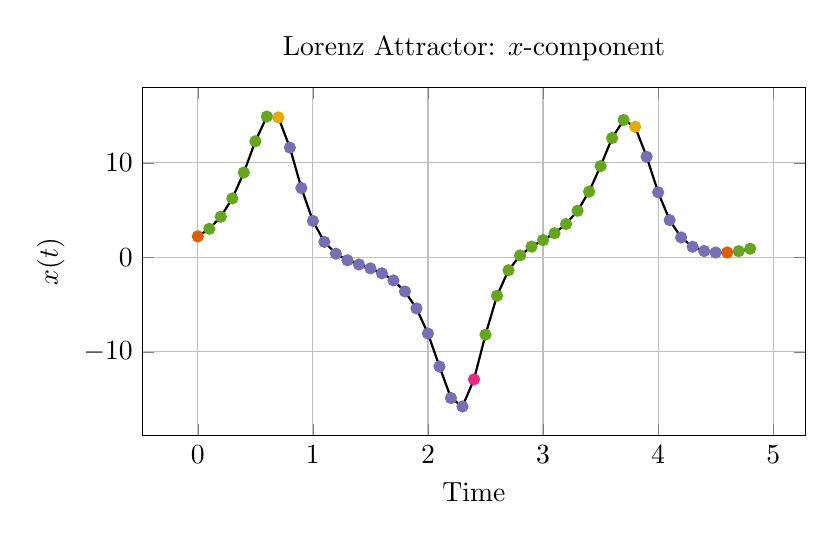
\begin{tikzpicture}
    \begin{axis}[
        xlabel={Time},
        ylabel={$x(t)$},
        title={Lorenz Attractor: $x$-component},
        width=10cm, height=6cm,
        grid=major
    ]


    \addplot [
        thick, % or any style you like
    ] coordinates {
        (0.0, 2.2165566502619796)
        (0.1, 3.0181360987381685)
        (0.2, 4.2948078524935065)
        (0.3, 6.231121537780632)
        (0.4, 8.970926893912857)
        (0.5, 12.272230400810887)
        (0.6, 14.887997312478161)
        (0.7, 14.803117347063516)
        (0.8, 11.606868473299526)
        (0.9, 7.330990437181266)
        (1.0, 3.85191889651296)
        (1.1, 1.6347534154776406)
        (1.2, 0.3853895148599277)
        (1.3, -0.30838099414996695)
        (1.4, -0.7586726217449103)
        (1.5, -1.1695821908357407)
        (1.6, -1.6858338981790886)
        (1.7, -2.443141458426554)
        (1.8, -3.6086854451117074)
        (1.9, -5.40339197322587)
        (2.0, -8.058505977971057)
        (2.1, -11.547145254692042)
        (2.2, -14.884182443761347)
        (2.3, -15.775516623377253)
        (2.4, -12.908181797239536)
        (2.5, -8.181376578133673)
        (2.6, -4.06724026097539)
        (2.7, -1.3665393788429014)
        (2.8, 0.20110496364168012)
        (2.9, 1.1324784341364973)
        (3.0, 1.8245674314417792)
        (3.1, 2.5516132966355554)
        (3.2, 3.5214281335608555)
        (3.3, 4.926987945369609)
        (3.4, 6.951562500713474)
        (3.5, 9.654345729238477)
        (3.6, 12.617195234374243)
        (3.7, 14.521825487882024)
        (3.8, 13.806356286601272)
        (3.9, 10.64113968132102)
        (4.0, 6.880279139891668)
        (4.1, 3.9367704788159394)
        (4.2, 2.1029851064946445)
        (4.3, 1.121305395878461)
        (4.4, 0.665491176850325)
        (4.5, 0.5051437108082056)
        (4.6, 0.5156168027361644)
        (4.7, 0.6490783162490397)
        (4.8, 0.9105168761220792)
    };
    
    
    % Define how each "class" (symbolic label) is colored and drawn:
    \addplot[
        scatter,
        only marks,
        scatter src=explicit symbolic,
        scatter/classes={
            1={mark=*,draw=col1,fill=col1},
            2={mark=*,draw=col2,fill=col2},
            3={mark=*,draw=col3,fill=col3},
            4={mark=*,draw=col4,fill=col4},
            5={mark=*,draw=col5,fill=col5},
            6={mark=*,draw=col6,fill=col6}
        }
    ] 
    coordinates {
        (0.0, 2.2165566502619796)[2]
        (0.1, 3.0181360987381685)[5]
        (0.2, 4.2948078524935065)[5]
        (0.3, 6.231121537780632)[5]
        (0.4, 8.970926893912857)[5]
        (0.5, 12.272230400810887)[5]
        (0.6, 14.887997312478161)[5]
        (0.7, 14.803117347063516)[6]
        (0.8, 11.606868473299526)[1]
        (0.9, 7.330990437181266)[1]
        (1.0, 3.85191889651296)[1]
        (1.1, 1.6347534154776406)[1]
        (1.2, 0.3853895148599277)[1]
        (1.3, -0.30838099414996695)[1]
        (1.4, -0.7586726217449103)[1]
        (1.5, -1.1695821908357407)[1]
        (1.6, -1.6858338981790886)[1]
        (1.7, -2.443141458426554)[1]
        (1.8, -3.6086854451117074)[1]
        (1.9, -5.40339197322587)[1]
        (2.0, -8.058505977971057)[1]
        (2.1, -11.547145254692042)[1]
        (2.2, -14.884182443761347)[1]
        (2.3, -15.775516623377253)[1]
        (2.4, -12.908181797239536)[4]
        (2.5, -8.181376578133673)[5]
        (2.6, -4.06724026097539)[5]
        (2.7, -1.3665393788429014)[5]
        (2.8, 0.20110496364168012)[5]
        (2.9, 1.1324784341364973)[5]
        (3.0, 1.8245674314417792)[5]
        (3.1, 2.5516132966355554)[5]
        (3.2, 3.5214281335608555)[5]
        (3.3, 4.926987945369609)[5]
        (3.4, 6.951562500713474)[5]
        (3.5, 9.654345729238477)[5]
        (3.6, 12.617195234374243)[5]
        (3.7, 14.521825487882024)[5]
        (3.8, 13.806356286601272)[6]
        (3.9, 10.64113968132102)[1]
        (4.0, 6.880279139891668)[1]
        (4.1, 3.9367704788159394)[1]
        (4.2, 2.1029851064946445)[1]
        (4.3, 1.121305395878461)[1]
        (4.4, 0.665491176850325)[1]
        (4.5, 0.5051437108082056)[1]
        (4.6, 0.5156168027361644)[2]
        (4.7, 0.6490783162490397)[5]
        (4.8, 0.9105168761220792)[5]
    };
    
    \end{axis}
    \end{tikzpicture}
    \caption{this is the caption}
    \label{fig:labelhere}
\end{figure}

\begin{table}[]
    \centering
    \begin{tabular}{c|cccccc}
        & \tikz\draw[fill=col1,draw=col1] (0,0) circle (0.9ex); 
        & \tikz\draw[fill=col2,draw=col2] (0,0) circle (0.9ex); 
        & \tikz\draw[fill=col3,draw=col3] (0,0) circle (0.9ex); 
        & \tikz\draw[fill=col4,draw=col4] (0,0) circle (0.9ex); 
        & \tikz\draw[fill=col5,draw=col5] (0,0) circle (0.9ex); 
        & \tikz\draw[fill=col6,draw=col6] (0,0) circle (0.9ex); \\ \hline
        \tikz\draw[fill=col1,draw=col1] (0,0) circle (0.9ex); & 0.7 & 0.1 & 0.1 & 0.05 & 0.05 & 0.0 \\
        \tikz\draw[fill=col2,draw=col2] (0,0) circle (0.9ex); & 0.0 & 0.0 & 0.0 & 0.0 & 0.9 & 0.1 \\
        \tikz\draw[fill=col3,draw=col3] (0,0) circle (0.9ex); & 0.7 & 0.1 & 0.1 & 0.05 & 0.05 & 0.0 \\
        \tikz\draw[fill=col4,draw=col4] (0,0) circle (0.9ex); & 0.0 & 0.0 & 0.0 & 0.0 & 0.9 & 0.1 \\
        \tikz\draw[fill=col5,draw=col5] (0,0) circle (0.9ex); & 0.0 & 0.0 & 0.0 & 0.0 & 0.9 & 0.1 \\
        \tikz\draw[fill=col6,draw=col6] (0,0) circle (0.9ex); & 0.7 & 0.05 & 0.05 & 0.05 & 0.05 & 0.1 \\
    \end{tabular}
    \caption{Transition probabilities between ordinal partitions.}
    \label{tab:transition_probabilities}
\end{table}

% !TEX root = ../HonoursThesisTemplate.tex

\chapter{Echo State Network with Ordinal Partition based readout switching}


Switch the readout ($C_{out}$) vector based on the ordinal partition.

When fitting the readout vectors, for each partition $p$:
\[
    (\mathbf{C_{out}})_p = (\mathbf{S}_p^T \mathbf{S}_p + \beta \mathbf{I}) \ \mathbf{S}_p^T \mathbf{Y}_p
\]
Where
\begin{itemize}
    \item $\mathbf{S}_p$ is $\mathbf{S}$ filtered to the states that results from data points with partition $p$. 
    \item $\mathbf{Y}_{p}$ is $\mathbf{Y}$ filtered to data points that follow immediately from data points with partition $p$.
\end{itemize}
And when infering the prediction at partition $p$:
\[
    \mathbf{y}(t) = (\mathbf{C}_{out})_{P(t)}\mathbf{s}(t)
\]
Where $P(t)$ is the partition of $x(t)$.

\begin{figure}
        
\centering
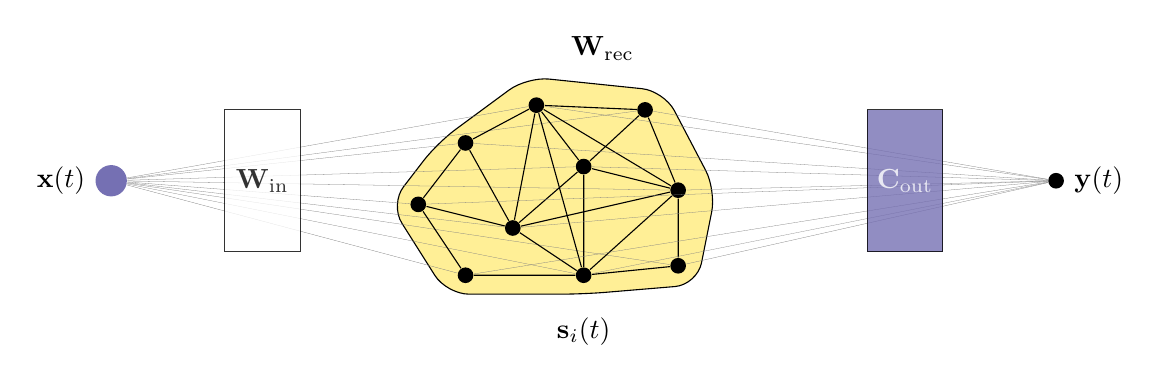
\begin{tikzpicture}[scale=1.2]
    \node[fill=col1,circle,inner sep=4pt,label=left:$\mathbf{x}(t)$] (input) at (0,0) {};
    \node[fill=black,circle,inner sep=2pt,label=right:$\mathbf{y}(t)$] (output) at (10,0) {};
    
    
    \coordinate (res_anchor) at (2,3);
    \node[fill=black,circle,inner sep=2pt] (res1) at ({5-0.5},{0.8}) {};
    \node[fill=black,circle,inner sep=2pt] (res2) at ({5},{-1}) {};
    \node[fill=black,circle,inner sep=2pt] (res3) at ({5},{0.15}) {};
    \node[fill=black,circle,inner sep=2pt] (res4) at ({5+1},{-0.1}) {};
    \node[fill=black,circle,inner sep=2pt] (res5) at ({5-0.75},{-0.5}) {};
    \node[fill=black,circle,inner sep=2pt] (res6) at ({5-1.25},{0.4}) {};
    \node[fill=black,circle,inner sep=2pt] (res7) at ({5+0.65},{0.75}) {};
    \node[fill=black,circle,inner sep=2pt] (res8) at ({5+1},{-0.9}) {};
    \node[fill=black,circle,inner sep=2pt] (res9) at ({5-1.25},{-1}) {};
    \node[fill=black,circle,inner sep=2pt] (res10) at ({5-1.75},{-0.25}) {};

    \foreach \i in {1,...,10}
        \draw[gray,line width=0.1] (input) -- (res\i);
    
    \foreach \i in {1,...,5}
        \foreach \j in {1,...,5} {
            \ifnum\i<\j
                \draw (res\i) -- (res\j);
            \fi
        }
    
    \draw (res6) -- (res5);
    \draw (res6) -- (res1);
    \draw (res6) -- (res10);
    \draw (res10) -- (res5);
    \draw (res9) -- (res10);
    \draw (res9) -- (res2);
    \draw (res7) -- (res1);
    \draw (res7) -- (res3);
    \draw (res7) -- (res4);
    \draw (res8) -- (res4);
    \draw (res8) -- (res2);
    
    \foreach \i in {1,...,10}
        \draw[gray,line width=0.1] (res\i) -- (output);
    
    \begin{scope}[on background layer]
    \draw[draw=black,fill=pale_yellow,rounded corners=8pt]  ($(res1)+(-0.1,0.3)$) -- ($(res7)+(+0.2,+0.2)$) -- ($(res4)+(0.4,0)$) -- ($(res8)+(0.2,-0.2)$) -- ($(res2)+(0,-0.2)$) -- ($(res9)+(-0.2,-0.2)$) -- ($(res10)+(-0.3,0)$) -- ($(res6)+(-0.3,0)$) -- cycle;
    \end{scope}
    \node at (5.2, 1.4) {$\mathbf{W}_{\text{rec}}$};
    \node at (5, -1.6) {$\mathbf{s}_i(t)$};
    
    \draw[fill=white,opacity=0.8] (1.2,-0.75) rectangle (2.0,0.75) node[midway] {$\mathbf{W}_{\text{in}}$};
    \draw[fill=col1,opacity=0.8] (8, -0.75) rectangle (8.8,0.75) node[midway, text=white] {$\mathbf{C}_{\text{out}}$};
\end{tikzpicture}

    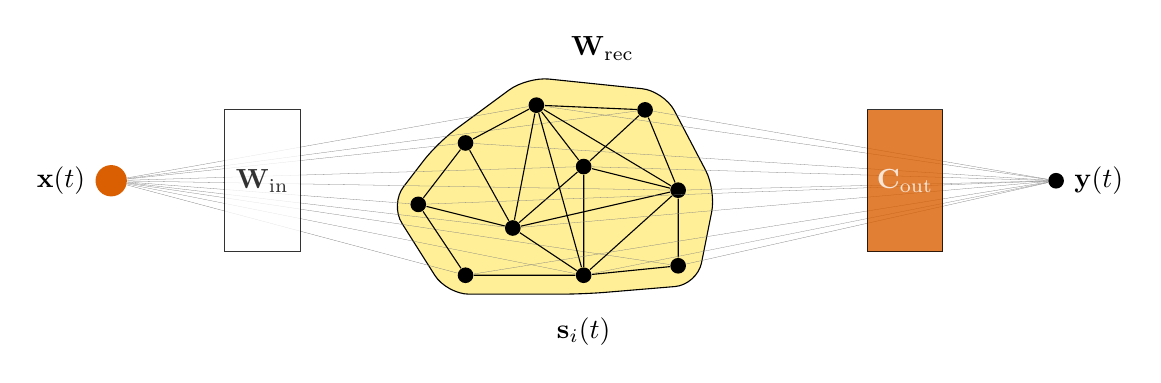
\begin{tikzpicture}[scale=1.2]
        \node[fill=col2,circle,inner sep=4pt,label=left:$\mathbf{x}(t)$] (input) at (0,0) {};
        \node[fill=black,circle,inner sep=2pt,label=right:$\mathbf{y}(t)$] (output) at (10,0) {};
        
        
        \coordinate (res_anchor) at (2,3);
        \node[fill=black,circle,inner sep=2pt] (res1) at ({5-0.5},{0.8}) {};
        \node[fill=black,circle,inner sep=2pt] (res2) at ({5},{-1}) {};
        \node[fill=black,circle,inner sep=2pt] (res3) at ({5},{0.15}) {};
        \node[fill=black,circle,inner sep=2pt] (res4) at ({5+1},{-0.1}) {};
        \node[fill=black,circle,inner sep=2pt] (res5) at ({5-0.75},{-0.5}) {};
        \node[fill=black,circle,inner sep=2pt] (res6) at ({5-1.25},{0.4}) {};
        \node[fill=black,circle,inner sep=2pt] (res7) at ({5+0.65},{0.75}) {};
        \node[fill=black,circle,inner sep=2pt] (res8) at ({5+1},{-0.9}) {};
        \node[fill=black,circle,inner sep=2pt] (res9) at ({5-1.25},{-1}) {};
        \node[fill=black,circle,inner sep=2pt] (res10) at ({5-1.75},{-0.25}) {};
    
        \foreach \i in {1,...,10}
            \draw[gray,line width=0.1] (input) -- (res\i);
        
        \foreach \i in {1,...,5}
            \foreach \j in {1,...,5} {
                \ifnum\i<\j
                    \draw (res\i) -- (res\j);
                \fi
            }
        
        \draw (res6) -- (res5);
        \draw (res6) -- (res1);
        \draw (res6) -- (res10);
        \draw (res10) -- (res5);
        \draw (res9) -- (res10);
        \draw (res9) -- (res2);
        \draw (res7) -- (res1);
        \draw (res7) -- (res3);
        \draw (res7) -- (res4);
        \draw (res8) -- (res4);
        \draw (res8) -- (res2);
        
        \foreach \i in {1,...,10}
            \draw[gray,line width=0.1] (res\i) -- (output);
        
        \begin{scope}[on background layer]
        \draw[draw=black,fill=pale_yellow,rounded corners=8pt]  ($(res1)+(-0.1,0.3)$) -- ($(res7)+(+0.2,+0.2)$) -- ($(res4)+(0.4,0)$) -- ($(res8)+(0.2,-0.2)$) -- ($(res2)+(0,-0.2)$) -- ($(res9)+(-0.2,-0.2)$) -- ($(res10)+(-0.3,0)$) -- ($(res6)+(-0.3,0)$) -- cycle;
        \end{scope}
        \node at (5.2, 1.4) {$\mathbf{W}_{\text{rec}}$};
        \node at (5, -1.6) {$\mathbf{s}_i(t)$};
        
        \draw[fill=white,opacity=0.8] (1.2,-0.75) rectangle (2.0,0.75) node[midway] {$\mathbf{W}_{\text{in}}$};
        \draw[fill=col2,opacity=0.8] (8, -0.75) rectangle (8.8,0.75) node[midway, text=white] {$\mathbf{C}_{\text{out}}$};
    \end{tikzpicture}
    \caption{Echo State Network with readout switching.}
    \label{fig:ESN}
\end{figure}
% !TEX root = ../HonoursThesisTemplate.tex

\chapter{Echo State Network with Ordinal Partition based Sub-Reservoirs}

\begin{itemize}
    \item Restructure the reservoir into `subreservoirs' for each partition.
    \item Feed the input based on the ordinal partition.
    \item Weight the connections between subreservoirs according to the ordinal transition probabilities.
\end{itemize}

\begin{figure}
        
    \centering
    \begin{tikzpicture}%[scale=0.8]
        \node[fill=col1,circle,inner sep=4pt,label=left:$\mathbf{x}(t)$] (input) at (0,0) {};
        \node[fill=black,circle,inner sep=2pt,label=right:$\mathbf{y}(t)$] (output) at (10,0) {};
        


        % Layer 1
        
        % The nodes of the reservoir
        \coordinate (res_anchor) at (5,3);
        \node[fill=black,circle,inner sep=2pt] (res1) at ($(res_anchor) + (-0.5,0.8)$) {};
        \node[fill=black,circle,inner sep=2pt] (res2) at ($(res_anchor) + (0,-1)$) {};
        \node[fill=black,circle,inner sep=2pt] (res3) at ($(res_anchor) + (0,0.15)$) {};
        \node[fill=black,circle,inner sep=2pt] (res4) at ($(res_anchor) + (1,-0.1)$) {};
        \node[fill=black,circle,inner sep=2pt] (res5) at ($(res_anchor) + (-0.75,-0.5)$) {};
        \node[fill=black,circle,inner sep=2pt] (res6) at ($(res_anchor) + (-1.25,0.4)$) {};
        \node[fill=black,circle,inner sep=2pt] (res7) at ($(res_anchor) + (0.65,0.75)$) {};
        \node[fill=black,circle,inner sep=2pt] (res8) at ($(res_anchor) + (1,-0.9)$) {};
        \node[fill=black,circle,inner sep=2pt] (res9) at ($(res_anchor) + (-1.25,-1)$) {};
        \node[fill=black,circle,inner sep=2pt] (res10) at ($(res_anchor) + (-1.75,-0.25)$) {};
        
        % The internal connections in the reservoir
        \foreach \i in {1,...,5}
            \foreach \j in {1,...,5} {
                \ifnum\i<\j
                    \draw (res\i) -- (res\j);
                \fi
            }
        
        % More internal connections in the reservoir
        \draw (res6) -- (res5);
        \draw (res6) -- (res1);
        \draw (res6) -- (res10);
        \draw (res10) -- (res5);
        \draw (res9) -- (res10);
        \draw (res9) -- (res2);
        \draw (res7) -- (res1);
        \draw (res7) -- (res3);
        \draw (res7) -- (res4);
        \draw (res8) -- (res4);
        \draw (res8) -- (res2);
        
        % Reservoir background
        \begin{scope}[on background layer]
        \draw[draw=black,fill=col1_light,rounded corners=8pt]  ($(res1)+(-0.1,0.3)$) -- ($(res7)+(+0.2,+0.2)$) -- ($(res4)+(0.4,0)$) -- ($(res8)+(0.2,-0.2)$) -- ($(res2)+(0,-0.2)$) -- ($(res9)+(-0.2,-0.2)$) -- ($(res10)+(-0.3,0)$) -- ($(res6)+(-0.3,0)$) -- cycle;
        \end{scope}

        % Layer 2

        % The nodes of the reservoir
        \coordinate (res_anchor) at (5,0);
        \node[fill=black,circle,inner sep=2pt] (res11) at ($(res_anchor) + (-0.5,0.8)$) {};
        \node[fill=black,circle,inner sep=2pt] (res12) at ($(res_anchor) + (0,-1)$) {};
        \node[fill=black,circle,inner sep=2pt] (res13) at ($(res_anchor) + (0,0.15)$) {};
        \node[fill=black,circle,inner sep=2pt] (res14) at ($(res_anchor) + (1,-0.1)$) {};
        \node[fill=black,circle,inner sep=2pt] (res15) at ($(res_anchor) + (-0.75,-0.5)$) {};
        \node[fill=black,circle,inner sep=2pt] (res16) at ($(res_anchor) + (-1.25,0.4)$) {};
        \node[fill=black,circle,inner sep=2pt] (res17) at ($(res_anchor) + (0.65,0.75)$) {};
        \node[fill=black,circle,inner sep=2pt] (res18) at ($(res_anchor) + (1,-0.9)$) {};
        \node[fill=black,circle,inner sep=2pt] (res19) at ($(res_anchor) + (-1.25,-1)$) {};
        \node[fill=black,circle,inner sep=2pt] (res20) at ($(res_anchor) + (-1.75,-0.25)$) {};
        
        % The internal connections in the reservoir
        \foreach \i in {16,...,20}
            \foreach \j in {16,...,20} {
                \ifnum\i<\j
                    \draw (res\i) -- (res\j);
                \fi
            }
        
        % More internal connections in the reservoir
        \draw (res16) -- (res15);
        \draw (res16) -- (res11);
        % \draw (res16) -- (res20);
        % \draw (res20) -- (res15);
        % \draw (res19) -- (res20);
        % \draw (res19) -- (res12);
        % \draw (res17) -- (res11);
        % \draw (res17) -- (res13);
        % \draw (res17) -- (res14);
        % \draw (res18) -- (res14);
        % \draw (res18) -- (res12);
        
        % Reservoir background
        \begin{scope}[on background layer]
        \draw[draw=black,fill=col2_light,rounded corners=8pt]  ($(res11)+(-0.1,0.3)$) -- ($(res17)+(+0.2,+0.2)$) -- ($(res14)+(0.4,0)$) -- ($(res18)+(0.2,-0.2)$) -- ($(res12)+(0,-0.2)$) -- ($(res19)+(-0.2,-0.2)$) -- ($(res20)+(-0.3,0)$) -- ($(res16)+(-0.3,0)$) -- cycle;
        \end{scope}

        % Layer 3

        % The nodes of the reservoir
        \coordinate (res_anchor) at (5,-3);
        \node[fill=black,circle,inner sep=2pt] (res21) at ($(res_anchor) + (-0.5,0.8)$) {};
        \node[fill=black,circle,inner sep=2pt] (res22) at ($(res_anchor) + (0,-1)$) {};
        \node[fill=black,circle,inner sep=2pt] (res23) at ($(res_anchor) + (0,0.15)$) {};
        \node[fill=black,circle,inner sep=2pt] (res24) at ($(res_anchor) + (1,-0.1)$) {};
        \node[fill=black,circle,inner sep=2pt] (res25) at ($(res_anchor) + (-0.75,-0.5)$) {};
        \node[fill=black,circle,inner sep=2pt] (res26) at ($(res_anchor) + (-1.25,0.4)$) {};
        \node[fill=black,circle,inner sep=2pt] (res27) at ($(res_anchor) + (0.65,0.75)$) {};
        \node[fill=black,circle,inner sep=2pt] (res28) at ($(res_anchor) + (1,-0.9)$) {};
        \node[fill=black,circle,inner sep=2pt] (res29) at ($(res_anchor) + (-1.25,-1)$) {};
        \node[fill=black,circle,inner sep=2pt] (res30) at ($(res_anchor) + (-1.75,-0.25)$) {};
        
        % The internal connections in the reservoir
        \foreach \i in {24,...,28}
            \foreach \j in {24,...,28} {
                \ifnum\i<\j
                    \draw (res\i) -- (res\j);
                \fi
            }
        
        % More internal connections in the reservoir
        % \draw (res26) -- (res25);
        % \draw (res26) -- (res21);
        \draw (res26) -- (res30);
        \draw (res30) -- (res25);
        \draw (res29) -- (res30);
        \draw (res29) -- (res22);
        % \draw (res27) -- (res21);
        % \draw (res27) -- (res23);
        % \draw (res27) -- (res24);
        % \draw (res28) -- (res24);
        % \draw (res28) -- (res22);
        
        % Reservoir background
        \begin{scope}[on background layer]
        \draw[draw=black,fill=col3_light,rounded corners=8pt]  ($(res21)+(-0.1,0.3)$) -- ($(res27)+(+0.2,+0.2)$) -- ($(res24)+(0.4,0)$) -- ($(res28)+(0.2,-0.2)$) -- ($(res22)+(0,-0.2)$) -- ($(res29)+(-0.2,-0.2)$) -- ($(res30)+(-0.3,0)$) -- ($(res26)+(-0.3,0)$) -- cycle;
        \end{scope}

        % Dotted connections between layers
        \foreach \i in {1,...,10} {
            \pgfmathtruncatemacro{\j}{\i+10}
            \pgfmathtruncatemacro{\k}{\i+20}
            \draw[dotted] (res\i) -- (res\j);
            \draw[dotted] (res\i) -- (res\k);
            \draw[dotted] (res\j) -- (res\k);
        }


        % The input connections
        \foreach \i in {1,...,10}
            \draw[gray,line width=0.1, path fading=fadeRL] (input) -- (res\i);
        
        % Output connections
        \foreach \i in {1,...,30} {
            \draw[gray, line width=0.1, path fading=fadeLR] (res\i) -- (output);
        }

        \draw[fill=white,opacity=0.8] (1.2,0.25) rectangle (2.0,1.75) node[midway] {$\mathbf{W}_{\text{in}}$};
        \draw[fill=white,opacity=0.8] (8, -0.75) rectangle (8.8,0.75) node[midway] {$\mathbf{C}_{\text{out}}$};
    \end{tikzpicture}
    \caption{Ordinally Partitioned Echo State Network.}
    \label{fig:ESN}
\end{figure}

For example, consider a partitioned Echo State Network with $3$ partitions (not actually possible).
    
With 3 partitions, the time series has the following transition probabilities:

\begin{table}[]
    \centering
    \begin{tabular}{c|cccccc}
        & \tikz\draw[fill=col1,draw=col1] (0,0) circle (0.9ex); 
        & \tikz\draw[fill=col2,draw=col2] (0,0) circle (0.9ex); 
        & \tikz\draw[fill=col3,draw=col3] (0,0) circle (0.9ex); \\ \hline
        \tikz\draw[fill=col1,draw=col1] (0,0) circle (0.9ex); & 0.7 & 0.1 & 0.2 \\
        \tikz\draw[fill=col2,draw=col2] (0,0) circle (0.9ex); & 0.9 & 0.1 & 0 \\
        \tikz\draw[fill=col3,draw=col3] (0,0) circle (0.9ex); & 0.1 & 0 & 0.8
    \end{tabular}
    \label{tab:transition_probabilities}
    \caption{Example transition probabilities}
\end{table}
    









    Let $k_{part}$ be the number of nodes in each partition's sub reservoir,
    and let $\mathbf{W}_{p,q}$ refer to the submatrix of $\mathbf{W}_{rec}$ with indices:
    
    \begin{align*}
        \text{Rows:}\quad& \{ pk_{part} + 1, pk_{part} + 2, \dots, (p+1)k_{part} \} \\
        \text{Columns:}\quad& \{ qk_{part} + 1, qk_{part} + 2, \dots, (q+1)k_{part} \}
    \end{align*}
    

    % Then, we define \(\mathbf{W}_{rec}\) in block form as \(\mathbf{W}_{p,q}\), where each block \(\mathbf{W}_{p,q}\) is the submatrix of \(\mathbf{W}_{rec}\) whose rows are in \(\Omega_p\) and columns are in \(\Omega_q\). The weight matrix is then given by:
    Then $\mathbf{W}_{rec}$ is given by:

    \[
    \mathbf{W}_{p,q} =
    \begin{cases}
    \mathbf{I} P(p,q), & p \neq q, \\
    \mathbf{W}_{ER}, & p = q,
    \end{cases}
    \]

    where 
    \begin{itemize}
        \item \(\mathbf{I}\) is the \( k_{part} \times k_{part} \) identity matrix
        \item \( P(p,q) \) is the probability of transitioning from partition \( p \) to partition \( q \)
        \item $\mathbf{W}_{ER}$ is an Erdos-Renyi randomly instantiated network.
    \end{itemize}
    








    Example:

    For a $k_{layer}$ of $4$ and $3$ partitions (not actually possible).

    \begin{center}
    $W_{rec} = $
    \[
    \scalebox{0.75}{$
    \begin{bmatrix}
    0.12 & 0 & 0.34 & -0.67 & 0.78 & 0 & -0.23 & 0.11 & -0.56 & 0 & 0.47 & 0 \\
    -0.44 & 0.23 & 0 & 0 & -0.76 & 0.54 & 0 & -0.34 & 0 & 0.56 & 0.89 & 0 \\
    0.23 & 0.78 & 0 & 0 & 0.34 & 0.89 & 0 & 0.45 & 0.67 & 0 & -0.89 & -0.75 \\
    0 & 0.34 & 0.89 & 0 & 0.23 & 0 & -0.67 & 0.12 & 0 & 0.56 & 0 & -0.78 \\
    0.67 & 0.12 & 0 & 0.45 & 0 & 0.78 & 0 & 0.89 & 0.12 & 0 & 0.23 & 0 \\
    0 & 0.56 & 0.89 & 0 & 0.23 & 0 & 0.67 & 0 & 0.34 & 0.78 & 0 & 0 \\
    0.45 & 0 & 0.89 & 0.23 & 0 & 0.56 & 0.78 & 0 & 0.12 & 0 & 0.45 & 0.1 \\
    0.78 & 0.12 & 0 & 0 & 0.34 & 0 & 0.45 & 0.56 & 0 & 0.89 & 0 & 0 \\
    0.89 & 0.23 & 0 & 0.56 & 0 & 0.89 & 0 & 0 & 0.34 & 0 & 0.78 & 0.24 \\
    0.34 & 0 & 0.78 & 0 & 0.12 & 0 & 0 & 0.67 & 0 & 0.12 & 0 & 0 \\
    0.78 & 0.12 & 0 & 0.34 & 0 & 0.78 & 0.89 & 0 & 0.23 & 0.56 & 0 & -0.95 \\
    0 & 0.89 & 0.23 & 0 & 0.56 & 0 & 0.89 & 0.12 & 0 & 0.34 & 0 & 0
    \end{bmatrix}
    $}
    \]
    \end{center}
    











    Example:
    
    For a $k_{layer}$ of $4$ and $3$ partitions (not actually possible).

    \begin{center}
    $W_{rec} = $
    \[
    \scalebox{0.75}{$
    \begin{bmatrix}
    0.12 & 0 & 0.34 & -0.67 & 0 & 0 & 0 & 0 & 0 & 0 & 0 & 0 \\
    -0.44 & 0.23 & 0 & 0 & 0 & 0 & 0 & 0 & 0 & 0 & 0 & 0 \\
    0.23 & 0.78 & 0 & 0 & 0 & 0 & 0 & 0 & 0 & 0 & 0 & 0 \\
    0 & 0.34 & 0.89 & 0 & 0 & 0 & 0 & 0 & 0 & 0 & 0 & 0 \\
    0 & 0 & 0 & 0 & 0 & 0.78 & 0 & 0.89 & 0 & 0 & 0 & 0 \\
    0 & 0 & 0 & 0 & 0.23 & 0 & 0.67 & 0 & 0 & 0 & 0 & 0 \\
    0 & 0 & 0 & 0 & 0 & 0.56 & 0.78 & 0 & 0 & 0 & 0 & 0 \\
    0 & 0 & 0 & 0 & 0.34 & 0 & 0.45 & 0.56 & 0 & 0 & 0 & 0 \\
    0 & 0 & 0 & 0 & 0 & 0 & 0 & 0 & 0.34 & 0 & 0.78 & 0.24 \\
    0 & 0 & 0 & 0 & 0 & 0 & 0 & 0 & 0 & 0.12 & 0 & 0 \\
    0 & 0 & 0 & 0 & 0 & 0 & 0 & 0 & 0.23 & 0.56 & 0 & -0.95 \\
    0 & 0 & 0 & 0 & 0 & 0 & 0 & 0 & 0 & 0.34 & 0 & 0
    \end{bmatrix}
    $}
    \]
    \end{center}
    









    Example:
    
    For a $k_{layer}$ of $4$ and $3$ partitions (not actually possible).

    \begin{center}
    $W_{rec} = $
    \[
    \scalebox{0.75}{$
    \begin{bmatrix}
        0.12 & 0 & 0.34 & -0.67 & 0.1 & 0 & 0 & 0 & 0.2 & 0 & 0 & 0 \\
        -0.44 & 0.23 & 0 & 0 & 0 & 0.1 & 0 & 0 & 0 & 0.2 & 0 & 0 \\
        0.23 & 0.78 & 0 & 0 & 0 & 0 & 0.1 & 0 & 0 & 0 & 0.2 & 0 \\
        0 & 0.34 & 0.89 & 0 & 0 & 0 & 0 & 0.1 & 0 & 0 & 0 & 0.2 \\
        0.9 & 0 & 0 & 0 & 0 & 0.78 & 0 & 0.89 & 0 & 0 & 0 & 0 \\
        0 & 0.9 & 0 & 0 & 0.23 & 0 & 0.67 & 0 & 0 & 0 & 0 & 0 \\
        0 & 0 & 0.9 & 0 & 0 & 0.56 & 0.78 & 0 & 0 & 0 & 0 & 0 \\
        0 & 0 & 0 & 0.9 & 0.34 & 0 & 0.45 & 0.56 & 0 & 0 & 0 & 0 \\
        0.1 & 0 & 0 & 0 & 0 & 0 & 0 & 0 & 0.34 & 0 & 0.78 & 0.24 \\
        0 & 0.1 & 0 & 0 & 0 & 0 & 0 & 0 & 0 & 0.12 & 0 & 0 \\
        0 & 0 & 0.1 & 0 & 0 & 0 & 0 & 0 & 0.23 & 0.56 & 0 & -0.95 \\
        0 & 0 & 0 & 0.1 & 0 & 0 & 0 & 0 & 0 & 0.34 & 0 & 0
    \end{bmatrix}
    $}
    \]
    \end{center}













    To only feed the input into the relevant layer, we mask all values of $\textbf{W}_{in}$ except those in the relevant partition.

    Given a randomly instantiated input vector $\textbf{W}_{all}$ of size $k_{part}O$ where $O$ is the number of partitions, we can define $\textbf{W}_{in}$ as a function of $p_t$, the partition of the input at time $t$:

    \[
        \textbf{W}_{in}(p_t)_i = \begin{cases}
            (\textbf{W}_{all})_i, & k_{part}(p_t-1) < i \leq k_{part}p_t\\
            0,                   & otherwise.
        \end{cases}
    \]

    % \begin{center}
    Example:
        \[
        \scalebox{0.75}{$
        \textbf{W}_{all} = \begin{bmatrix}
            0.12 & 0.5 & 0.34 & -0.67 & 0.1 & -0.43 & 0.98 & -0.64 & 0.2 & 0.45 & 0.2 & -0.45
        \end{bmatrix}
        $}
        \]
        \[
        \scalebox{0.75}{$
        \textbf{W}_{in}(1) = \begin{bmatrix}
            0.12 & 0.5 & 0.34 & -0.67 & 0 & 0 & 0 & 0 & 0 & 0 & 0 & 0
        \end{bmatrix}
        $}
        \]
        \[
        \scalebox{0.75}{$
        \textbf{W}_{in}(2) = \begin{bmatrix}
            0 & 0 & 0 & 0 & 0.1 & -0.43 & 0.98 & -0.64 & 0 & 0 & 0 & 0
        \end{bmatrix}
        $}
        \]
        \[
        \scalebox{0.75}{$
        \textbf{W}_{in}(3) = \begin{bmatrix}
            0 & 0 & 0 & 0 & 0 & 0 & 0 & 0 & 0.2 & 0.45 & 0.2 & -0.45
        \end{bmatrix}
        $}
        \]
    % \end{center}

% !TEX root = ../HonoursThesis.tex

\renewcommand{\chapterlabel}{Chapter}
\chapter{Echo state network with ordinal partition based readout switching}
\label{chap:ORSESN}


The first approach uses a piecewise readout function to incorporate ordinal partition information into the structure of an ESN. In this architecture there is a different readout vector for each observed ordinal partition and at each time step, a readout vector is chosen depending on the partition of the input data. We will refer to this architecture as the Ordinal partition based Readout Switching ESN (ORSESN).

% \begin{figure}
%     \centering
%     \begin{tikzpicture}[scale=1.2]
%         \node[fill=col1,circle,inner sep=4pt,label=left:$\mathbf{x}(t)$] (input) at (0,0) {};
%         \node[fill=black,circle,inner sep=2pt,label=right:$\mathbf{y}(t)$] (output) at (10,0) {};
        
        
%         \coordinate (res_anchor) at (2,3);
%         \node[fill=black,circle,inner sep=2pt] (res1) at ({5-0.5},{0.8}) {};
%         \node[fill=black,circle,inner sep=2pt] (res2) at ({5},{-1}) {};
%         \node[fill=black,circle,inner sep=2pt] (res3) at ({5},{0.15}) {};
%         \node[fill=black,circle,inner sep=2pt] (res4) at ({5+1},{-0.1}) {};
%         \node[fill=black,circle,inner sep=2pt] (res5) at ({5-0.75},{-0.5}) {};
%         \node[fill=black,circle,inner sep=2pt] (res6) at ({5-1.25},{0.4}) {};
%         \node[fill=black,circle,inner sep=2pt] (res7) at ({5+0.65},{0.75}) {};
%         \node[fill=black,circle,inner sep=2pt] (res8) at ({5+1},{-0.9}) {};
%         \node[fill=black,circle,inner sep=2pt] (res9) at ({5-1.25},{-1}) {};
%         \node[fill=black,circle,inner sep=2pt] (res10) at ({5-1.75},{-0.25}) {};

%         \foreach \i in {1,...,10}
%             \draw[gray,line width=0.1] (input) -- (res\i);
        
%         \foreach \i in {1,...,5}
%             \foreach \j in {1,...,5} {
%                 \ifnum\i<\j
%                     \draw (res\i) -- (res\j);
%                 \fi
%             }
        
%         \draw (res6) -- (res5);
%         \draw (res6) -- (res1);
%         \draw (res6) -- (res10);
%         \draw (res10) -- (res5);
%         \draw (res9) -- (res10);
%         \draw (res9) -- (res2);
%         \draw (res7) -- (res1);
%         \draw (res7) -- (res3);
%         \draw (res7) -- (res4);
%         \draw (res8) -- (res4);
%         \draw (res8) -- (res2);
        
%         \foreach \i in {1,...,10}
%             \draw[gray,line width=0.1] (res\i) -- (output);
        
%         \begin{scope}[on background layer]
%         \draw[draw=black,fill=pale_yellow,rounded corners=8pt]  ($(res1)+(-0.1,0.3)$) -- ($(res7)+(+0.2,+0.2)$) -- ($(res4)+(0.4,0)$) -- ($(res8)+(0.2,-0.2)$) -- ($(res2)+(0,-0.2)$) -- ($(res9)+(-0.2,-0.2)$) -- ($(res10)+(-0.3,0)$) -- ($(res6)+(-0.3,0)$) -- cycle;
%         \end{scope}
%         \node at (5.2, 1.4) {$\mathbf{W}_{\text{rec}}$};
%         \node at (5, -1.6) {$\mathbf{s}(t)$};
        
%         \draw[fill=white,opacity=0.8] (1.2,-0.75) rectangle (2.0,0.75) node[midway] {$\mathbf{W}_{\text{in}}$};
%         % \draw[fill=col3,opacity=0.8] (8, -0.75+2) rectangle (8.8,0.75+2) node[midway, text=white] {$\mathbf{C}_{\text{out}}$};
%         \draw[fill=col1,opacity=0.8] (8, -0.75) rectangle (8.8,0.75) node[midway, text=white] {$\mathbf{C}_{\text{out}}$};
%         % \draw[fill=col2,opacity=0.8] (8, -0.75-2) rectangle (8.8,0.75-2) node[midway, text=white] {$\mathbf{C}_{\text{out}}$};
%     \end{tikzpicture}

%     \begin{tikzpicture}[scale=1.2]
%         \node[fill=col2,circle,inner sep=4pt,label=left:$\mathbf{x}(t)$] (input) at (0,0) {};
%         \node[fill=black,circle,inner sep=2pt,label=right:$\mathbf{y}(t)$] (output) at (10,0) {};
        
        
%         \coordinate (res_anchor) at (2,3);
%         \node[fill=black,circle,inner sep=2pt] (res1) at ({5-0.5},{0.8}) {};
%         \node[fill=black,circle,inner sep=2pt] (res2) at ({5},{-1}) {};
%         \node[fill=black,circle,inner sep=2pt] (res3) at ({5},{0.15}) {};
%         \node[fill=black,circle,inner sep=2pt] (res4) at ({5+1},{-0.1}) {};
%         \node[fill=black,circle,inner sep=2pt] (res5) at ({5-0.75},{-0.5}) {};
%         \node[fill=black,circle,inner sep=2pt] (res6) at ({5-1.25},{0.4}) {};
%         \node[fill=black,circle,inner sep=2pt] (res7) at ({5+0.65},{0.75}) {};
%         \node[fill=black,circle,inner sep=2pt] (res8) at ({5+1},{-0.9}) {};
%         \node[fill=black,circle,inner sep=2pt] (res9) at ({5-1.25},{-1}) {};
%         \node[fill=black,circle,inner sep=2pt] (res10) at ({5-1.75},{-0.25}) {};

%         \foreach \i in {1,...,10}
%             \draw[gray,line width=0.1] (input) -- (res\i);
        
%         \foreach \i in {1,...,5}
%             \foreach \j in {1,...,5} {
%                 \ifnum\i<\j
%                     \draw (res\i) -- (res\j);
%                 \fi
%             }
        
%         \draw (res6) -- (res5);
%         \draw (res6) -- (res1);
%         \draw (res6) -- (res10);
%         \draw (res10) -- (res5);
%         \draw (res9) -- (res10);
%         \draw (res9) -- (res2);
%         \draw (res7) -- (res1);
%         \draw (res7) -- (res3);
%         \draw (res7) -- (res4);
%         \draw (res8) -- (res4);
%         \draw (res8) -- (res2);
        
%         \foreach \i in {1,...,10}
%             \draw[gray,line width=0.1] (res\i) -- (output);
        
%         \begin{scope}[on background layer]
%         \draw[draw=black,fill=pale_yellow,rounded corners=8pt]  ($(res1)+(-0.1,0.3)$) -- ($(res7)+(+0.2,+0.2)$) -- ($(res4)+(0.4,0)$) -- ($(res8)+(0.2,-0.2)$) -- ($(res2)+(0,-0.2)$) -- ($(res9)+(-0.2,-0.2)$) -- ($(res10)+(-0.3,0)$) -- ($(res6)+(-0.3,0)$) -- cycle;
%         \end{scope}
%         \node at (5.2, 1.4) {$\mathbf{W}_{\text{rec}}$};
%         \node at (5, -1.6) {$\mathbf{s}(t)$};
        
%         \draw[fill=white,opacity=0.8] (1.2,-0.75) rectangle (2.0,0.75) node[midway] {$\mathbf{W}_{\text{in}}$};
%         \draw[fill=col2,opacity=0.8] (8, -0.75) rectangle (8.8,0.75) node[midway, text=white] {$\mathbf{C}_{\text{out}}$};
%     \end{tikzpicture}
%     % \caption{echo state network with readout switching.}
%     \caption{Architecture of the Ordinal partition based Readout Switching ESN (ORSESN). Input $\mathbf{x}(t)$ is projected into a reservoir of $k=10$ nodes via $\mathbf{W}_{\mathrm{in}}$ and recurrently updated via $\mathbf{W}_{\mathrm{rec}}$. Partition specific readout vectors $\mathbf{C}_{\mathrm{out}}$ are selected based on the active ordinal partition, illustrated by colours purple and orange.}
%     \label{fig:readout_switching_ESN}
% \end{figure}

% TODO discuss Ma \& Chen (2013) and their state space partitioning and compare it to this case.

\section{Implementation}

\subsection{Instantiating the weights and iterating the reservoir}

The input weights $\mathbf{W}_{in}$ and recurrence matrix $\mathbf{W}_{rec}$ of the ORSESN are generated as they would be for a traditional ESN. $\mathbf{W}_{in}$ is a vector of length $k$ drawn from a Normal distribution and $\mathbf{W}_{rec}$ is an Erd\H{o}s-R\'enyi random network adjacency matrix. The initial states $s(0)$ form a vector of length $k$ and are initialised by drawing from a Normal distribution. The ORSESN can be driven with the input and the reservoir iterated just like a traditional ESN, using the update equation:

\[
    \mathbf{s}(t + 1) = f_{act}(\mathbf{W}_{in}\mathbf{x}(t) + \mathbf{W}_{rec}\mathbf{s}(t) + \mathbf{W}_{bias}).
\]

Driving the reservoir with the training sequence and collecting the states into a matrix $\mathbf{S}$ will prepare us to fit the vectors that make up the piecewise readout function. For a training sequence of length $n_{train}$, let us collect these states into a matrix:
\[
    \mathbf{S} = [\mathbf{s}(1), ..., \mathbf{s}(n_{train})]^t \in R^{n_{train}\times k}.
\]

\subsection{Fitting the readout vectors}

To fit the readout vector for each partition $\pi$, we must filter the input time series $\mathbf{Y}$ to those data points belonging to that partition $\pi$ and filter the states $\mathbf{S}$ to those that arose immediately after that input from that partition $\pi$. We can define those inputs $\mathbf{Y}_\pi$ and states $\mathbf{S}_{\pi}$ that relate to each partition $\pi$ by indexing $\mathbf{Y}$ and $\mathbf{S}$, where $\pi_t$ represents the ordinal partition of the data at time $t$:
\begin{align*}
    \mathbf{Y}_\pi &= \{\mathbf{Y}_{t} | \pi_t = \pi\}, \\
    \mathbf{S}_\pi &= \{\mathbf{S}_{t,*} | \pi_t = \pi\},
\end{align*}
and then for each partition $\pi$, we can fit a readout vector using Ridge regression:
\[
    (\mathbf{C}_{out}^T)_\pi = (\mathbf{S}_\pi^T \mathbf{S}_\pi + \beta \mathbf{I}) \ \mathbf{S}_\pi^T \mathbf{Y}_\pi.
\]
The readout vectors for each partition can then be arranged into an $N_{obs}\times k$ matrix,
\[
    \mathbf{C}_{out} = [(\mathbf{C}_{out})_1; ...; (\mathbf{C}_{out})_{N_{obs}}],
\]
and a vector of predictions for each possible partition $\mathbf{y}_{all}(t)$ at time $t$ can be inferred for any states $\mathbf{s}(t)$:
\[
    \mathbf{y}_{all}(t) = \mathbf{C}_{out}(t)\mathbf{s}(t).
\]

To obtain just one of these predictions, we construct a mask based on the active partition at each time step. This mask $e_\pi$ will be a `one-hot encoded' vector of length $N_{obs}$, where 1 indicates the active partition at that time step and 0 indicates the other inactive partitions. By multiplying our mask and the prediction vector and summing the result, we can select the prediction for a given ordinal partition $\pi_t$:
\[
    \mathbf{y}(t) = \sum \mathbf{y}_{all}(t)e_{\pi_t}.
\]

The selection of the prediction does not necessarily need to be one-hot like this, but could use an informed combination of predictions, as do other mixture-of-experts models~\cite{babinec_pospichal_2009}~\cite{laan_vicente_2015}. One such relevant method could be to weight the predictions of each of the partition readouts depending on the transition probabilities of the active ordinal partition, however we have not trialed this hypothesis.

Here we have defined a method for `switching' the readout of an ESN based on the ordinal partition of the input data.%Figure \ref{fig:readout_switching_ESN} visualises the switching of just the readout vector using the colour coding of ordinal partitions introduced in chapter \ref{chap:ordinal_partitions}.




\section{Results}



\subsection{Lorenz - iterative prediction}

First we will consider the mean RMSE created by iterative predictions of the Lorenz time series with a $\Delta t = 0.01$. At a single recursive prediction step, the traditional ESN achieves the lowest mean RMSE of 0.173 ($\pm 0.025$), outperforming the ORSESN for all ordinal pattern dimensions ($m$). For $m=2$, $3$, and $4$, the mean RMSEs are 0.237 ($\pm 0.015$), 0.258 ($\pm 0.012$), and 0.268 ($\pm 0.010$), respectively. This shows that for short term predictions, increasing the ordinal pattern dimension $m$ leads to a higher mean RMSE for the ORSESN, and that the traditional ESN is optimal for very short-term predictions. However, as the number of recursive prediction steps increases, this relationship changes. After two and three steps, the RMSEs for all models increase, but the gap between the traditional ESN and the ORSESN with higher $m$ begins to narrow. For example, at 3 steps, the traditional ESN has a mean RMSE of 0.334 ($\pm 0.055$), while the ORSESN with $m=4$ has a mean RMSE of 0.341 ($\pm 0.034$).

The significant change occurs at longer prediction horizons, as shown in Figure \ref{fig:ORSESN_iterative_0_01}. By 10 steps, the traditional ESN's mean RMSE rises to 1.093 ($\pm 0.159$), while the ORSESN with $m=4$ achieves a significantly lower (95\% CI) mean RMSE of 0.739 ($\pm 0.086$).
At 20 steps, the error rates have reversed: the traditional ESN's RMSE increases to 2.072 ($\pm 0.230$), whereas the ORSESN achieves significantly lower (95\% CI) errors for all $m$, with $m=4$ reaching the lowest RMSE of 1.004 ($\pm 0.092$). This advantage becomes even more pronounced as the prediction horizon extends further, with the ORSESN with $m=4$ achieving a mean RMSE of approximately 3.174 ($\pm 0.254$) at 70 steps compared to the traditional ESN's 6.915 ($\pm 0.732$). However for $m=2$, the trend does not significantly hold, with the $m=2$ ORSESN's mean RMSE failing to be significantly lower for most prediction horizons. The $m=3$ ORSESN ceases to provide a significant benefit at 200 prediction steps, beyond which all four models diverge from the signal.
These results demonstrate that, although the traditional ESN is best for immediate predictions, the ORSESN with higher ordinal pattern dimension $m$ provides significantly more accurate and stable predictions for longer prediction horizons.

The ORSESN also demonstrates greater consistency in its predictions compared to the traditional ESN, as measured by the standard deviation of RMSE across trials. Since each trial uses a newly instantiated set of states and weights, and regenerates the additive noise for the time series, the standard deviation of the RMSEs generated by each trial can represent how robust each architecture is to its random initial conditions. The ORSESN achieves a lower standard deviation of RMSE across trials, especially at longer prediction horizons. At 10 recursive steps, the traditional ESN shows a standard deviation of 0.159, while the ORSESN with $m=4$ has a much lower value of 0.086. This pattern continues at 30 steps (0.511 vs. 0.116) and 50 steps (0.679 vs. 0.147). Notably, the variability decreases as the ordinal pattern dimension increases, with $m=4$ consistently showing the lowest standard deviations in the medium-term prediction range.

When examining the Lorenz system with a larger time step size of $\Delta t=0.05$, we observe similar patterns although less pronounced. The traditional ESN has a mean RMSE of 1.330 ($\pm 0.040$) at a single prediction step, which is comparable to the ORSESN with $m=3$ (1.337 $\pm 0.055$) and $m=4$ (1.328 $\pm 0.059$). Compared to the Lorenz series with $\Delta t=0.01$, the performance of the ORSESN improves over the traditional ESN at even shorter prediction lengths. After just 2 recursive prediction steps, the ORSESN with $m=4$ already demonstrates significantly (95\% CI) superior performance with a mean RMSE of 1.483 ($\pm 0.040$) compared to the traditional ESN's 1.535 ($\pm 0.017$). The ORSESN with $m=3$ demonstrates significantly superior performance at 20 time steps, and $m=2$ at 30, but by 70 prediction steps, all three models have converged, as shown in Figure \ref{fig:ORSESN_iterative_0_05}.
% For 20 recursive prediction steps and beyond, the ORSESN models also showed consistently lower standard deviations.


\begin{figure}
    \centering

    \begin{subfigure}{\textwidth}
        \caption{Mean iterative prediction RMSE on the Lorenz series with time step size $\Delta t = 0.01$ for the ORSESN with delay $\tau=20$, noise level $\alpha=0.1$, and total reservoir size $k=500$.}
        \label{fig:ORSESN_iterative_0_01}
        \centering
        \makebox[\textwidth][c]{%
            \includegraphics[width=1.1\textwidth,trim=0 8mm 0 0,clip]{../Images/ORSESN/ORSESN_topline_recursive_Lorenz 0_01.pdf}
        }
    \end{subfigure}

    \vspace{0.5em}

    \begin{subfigure}{\textwidth}
        \caption{Mean iterative prediction RMSE on the Lorenz series with time step size $\Delta t=0.05$ for the ORSESN with delays $\tau=10,10,4$ for $m=2,3,4$ respectively, noise level $\alpha=0.1$, and total reservoir size $k=500$.}
        \label{fig:ORSESN_iterative_0_05}
        \centering
        \makebox[\textwidth][c]{%
            \includegraphics[width=1.1\textwidth]{../Images/ORSESN/ORSESN_topline_recursive_Lorenz 0_05.pdf}
        }
    \end{subfigure}

    % \caption{Mean iterative prediction RMSE for the ORSESN for Lorenz x component time series with two different time steps: (a) $\Delta t=0.01$ and (b) $\Delta t=0.05$, both with additive noise $\alpha=0.1$, delay $\tau=20$ and total reservoir size $k=468$. The standard deviations between trials are represented by vertical bars and the range of trial results is represented by the shaded regions.}
    \caption{Mean iterative prediction RMSE for the ORSESN on the Lorenz $x$-component time series with additive noise $\alpha=0.1$ and total reservoir size $k=500$. Subfigure (a) shows results for time step size $\Delta t=0.01$, delay $\tau=20$ for all $m$; subfigure (b) shows results for time step size $\Delta t=0.05$, delays $\tau=10,10,4$ for $m=2,3,4$, respectively. Standard deviations between trials are represented by vertical bars and shaded regions indicate the full range of trial results.}
\end{figure}



\subsection{Lorenz - direct prediction}


Here we will analyse the ability of the ORSESN to generate direct predictions. For the Lorenz system with time step size $\Delta t=0.01$, as shown in Figure \ref{fig:ORSESN_direct_0_01}, the traditional ESN initially performs well for short prediction horizons, achieving a mean RMSE of 0.228 ($\pm 0.033$) after 1 step. The ORSESN models show slightly higher errors at this prediction length, with mean RMSEs of 0.243 ($\pm 0.020$), 0.233 ($\pm 0.017$), and 0.228 ($\pm 0.021$) for $m=2$, $m=3$, and $m=4$, respectively. But mirroring what we observed in the iterative predictions, the ORSESN models perform better at longer prediction lengths. At 20 prediction steps, all three ORSESN models achieve a statistically significant (95\% CI) lower mean RMSE than the traditional ESN, with a higher $m$ producing a lower RMSE over the whole tested range of prediction lengths.

For direct prediction on the Lorenz system with time step size $\Delta t=0.05$ (Figure \ref{fig:ORSESN_direct_0_05}), the ORSESN with $m=4$ outperforms the traditional ESN from the start (mean RMSE of $0.239\pm 0.019$ vs. $0.311\pm 0.025$ at 1 step) and maintains this advantage throughout longer horizons ($0.759\pm 0.045$ vs. $1.175\pm 0.076$ at 5 steps; $5.003\pm 0.088$ vs. $6.214\pm 0.254$ at 20 steps). The ORSESN with $m=3$ also reliably outperforms the traditional ESN, however the ORSESN with $m=2$ fails to significantly improve (95\% CI) the traditional ESN at many prediction lengths.

Both direct and iterative prediction methods confirm the same conclusion: while traditional ESNs are superior or on-par for short-term forecasts, the ORSESN provides more accurate and stable predictions for medium to long-term horizons, with performance improving as the ordinal pattern dimension increases. The direct prediction results further confirm that the ORSESN's superior performance is not an artifact of error accumulation in iterative prediction but rather reflects a genuine improvement in the model's ability to capture the underlying dynamics of the chaotic system. There is a consistent pattern of lower errors for the ORSESN at longer prediction horizons across both forms of prediction.


\begin{figure}
    \centering

    \begin{subfigure}{\textwidth}
        \caption{Mean direct prediction RMSE on the Lorenz series with time step size $\Delta t=0.01$ for the ORSESN with delay $\tau=20$, noise level $\alpha=0.1$, and total reservoir size $k=500$.}
        \label{fig:ORSESN_direct_0_01}
        \centering
        \makebox[\textwidth][c]{%
            \includegraphics[width=1.1\textwidth,trim=0 8mm 0 0,clip]{../Images/ORSESN/ORSESN_topline_direct_Lorenz 0_01.pdf}
        }
    \end{subfigure}

    \vspace{0.5em}

    \begin{subfigure}{\textwidth}
        \caption{Mean direct prediction RMSE on the Lorenz series with time step size $\Delta t=0.05$ for the ORSESN with delay $\tau=4$, noise level $\alpha=0.1$, and total reservoir size $k=500$.}
        \label{fig:ORSESN_direct_0_05}
        \centering
        \makebox[\textwidth][c]{%
            \includegraphics[width=1.1\textwidth]{../Images/ORSESN/ORSESN_topline_direct_Lorenz 0_05.pdf}
        }
    \end{subfigure}

    \caption{Mean direct prediction RMSE for the ORSESN on the Lorenz $x$-component time series with additive noise $\alpha=0.1$ and total reservoir size $k=500$. Subfigure (a) shows results for time step size $\Delta t=0.01$, delay $\tau=20$ for all $m$; subfigure (b) shows results for time step size $\Delta t=0.05$, delay $\tau=4$ for all $m$. Standard deviations between trials are represented by vertical bars and shaded regions indicate the full range of trial results.}
    \label{fig:ORSESN_direct}
\end{figure}



\subsection{Comparison across attractors}

\subsubsection{R\"ossler system}

For the R\"ossler system integrated with a time step size of $\Delta t=0.1$ (Figure~\ref{fig:ORSESN_rossler_iterative}), the results show a similar pattern to the Lorenz attractor. The traditional ESN exhibits lower error for very short term predictions, but after 5 recursive steps the mean RMSE of the ORSESN with $m=4$ ($0.374 \pm 0.0190$) and $m=3$ ($0.385 \pm 0.022$) significantly (95\% CI) outperform the traditional ESN ($0.482 \pm 0.041$). Like those predictions for the Lorenz series, this advantage becomes more pronounced at longer horizons; for instance, at 200 steps, ORSESN with $m=4$ achieves a significantly lower mean RMSE of 2.176 ($\pm 0.250$) compared to 4.393 ($\pm 1.126$) for the traditional ESN. Furthermore, the ORSESN with $m=4$ demonstrates remarkable prediction stability at this horizon, with a standard deviation of only 0.250, whereas the traditional ESN has a standard deviation of 1.126.

The ORSESN with $m=2$ fails to be significantly more accurate at multiple prediction lengths, and the ORSESN with $m=3$ provides insignificant improvement after 150 prediction steps. After 200 prediction steps, the ORSESN with $m=4$ no longer significantly outperforms the traditional ESN, but this can be seen to be a result of the higher standard deviation in the results of the traditional ESN.

Comparing these findings with the Lorenz system, the general performance characteristics are consistent. Traditional ESNs tend to be more accurate for shorter prediction lengths, however ORSESN models outperform on accuracy and stability for longer predictions lengths, particularly where $m=4$.
The crossover point, where ORSESN models begin to outperform traditional ESNs, typically occurs within the first 10 prediction steps for both chaotic systems.

What appears peculiar is the comparably low mean RMSE and small variance of the ORSESN with $m=4$. Figure \ref{fig:ORSESN_rossler_freerun} shows iterative predictions over 200 prediction steps (Rossler with $\Delta t = 0.1$) for the ORSESN and traditional ESN. Simply inspecting these predictions, all four models appear to predict the dynamics of only approximately one cycle before reverting to an `average' periodic prediction. However the ORSESN with $m=4$ appears to be able to predict the dynamics of 2 to 3 cycles to varying degrees of success before reverting to the `average' periodic prediction.



\begin{figure}
    \centering

    \centering
    \makebox[\textwidth][c]{%
        \includegraphics[width=1.1\textwidth,trim=0 0 0 0,clip]{../Images/ORSESN/ORSESN_topline_recursive_rossler 0_1.pdf}
    }

    \caption{Mean iterative prediction RMSE for the ORSESN for R\"ossler $x$ component time series with time step size $\Delta t=0.1$ and additive noise $\alpha=0.1$, delay $\tau=20$ and total reservoir size $k=500$. The standard deviations between trials are represented by vertical bars and the range of trial results is represented by the shaded regions.}
    \label{fig:ORSESN_rossler_iterative}
\end{figure}

\begin{figure}
    \centering
    \makebox[\textwidth][c]{%
        \includegraphics[width=1\textwidth,trim=0 0 0 0,clip]{../Images/ORSESN/ORSESN_freerun_recursive_Rossler.pdf}
    }
    \caption{Iterative free-run predictions for the Rössler system ($x$ component) with time step size $\Delta t=0.1$. The figure compares the traditional ESN with ORSESN models of varying ordinal pattern dimensions ($m=2,3,4$) over 200 prediction steps. All models were configured with a delay $\tau=20$, additive noise $\alpha=0.1$, and a total reservoir size $k=500$. Each grey vertical line indicates the beginning of prediction chunk, where the echo state network changes from being driven by the true signal to being driven by its own predictions.}
    \label{fig:ORSESN_rossler_freerun}
\end{figure}



The direct prediction performance on the Rössler system (Figure \ref{fig:ORSESN_rossler_direct}) is consistent with the iterative prediction trends. The benefit of the ORSESN appears more pronounced for the Rossler time series than the Lorenz time series.
Direct predictions on the Rossler series again shows the traditional ESN with slightly lower error for short predictions but the ORSESN models with higher ordinal pattern dimensions ($m$) generally achieve better accuracy for longer predictions. At 20 prediction steps, ORSESN with $m=4$ (mean RMSE $0.701\pm 0.058$) is significantly (95\%CI) more accurate than the traditional ESN (mean RMSE $1.094\pm 0.155$).
The mean prediction RMSE for all models converges, similar to the direct predictions for the Lorenz series, at approximately 350 prediction steps.
% A prediction at this length simply reflects the ESN's ability to match the periodicity of the data rather than its ability to represent the dynamics of the attractor.


\begin{figure}

    \centering
    \makebox[\textwidth][c]{%
        \includegraphics[width=1.1\textwidth,trim=0 0 0 0,clip]{../Images/ORSESN/ORSESN_topline_direct_rossler 0_1.pdf}
    }

    \caption{Mean direct prediction RMSE for the ORSESN for R\"ossler $x$ component time series with time step size $\Delta t=0.1$ and additive noise $\alpha=0.1$, delay $\tau=20$ and total reservoir size $k=500$. The standard deviations between trials are represented by vertical bars and the range of trial results is represented by the shaded regions.}
    \label{fig:ORSESN_rossler_direct}
\end{figure}



\subsubsection{Mackey-Glass system}

% apple
The iterative prediction results for the Mackey-Glass system with a time step size $\Delta t=0.5$ are illustrated in Figure \ref{fig:ORSESN_mg_iterative}.
Like the Lorenz and R\"ossler attractors, the traditional ESN demonstrates a clear advantage in single time step prediction for this system.

Similarly again, the ORSESN models generally show significantly (95\% CI) improved performance over the traditional ESN as the prediction horizon grows. For instance, at 20 recursive prediction steps, the traditional ESN has a mean RMSE of 0.110 ($\pm 0.010$), while the ORSESN with $m=2$ achieves 0.071 ($\pm 0.003$), $m=3$: 0.070 ($\pm 0.003$), and $m=4$: 0.039 ($\pm 0.001$).

Unlike the other attractors, the ORSESN models with $m=2$ and $m=3$ maintain significantly (95\% CI) improved accuracy only up to around 70 prediction steps, while the ORSESN with $m=4$ continues to provide improved accuracy for much longer predictions.

The ORSESN with $m=4$ achieves a consistent significantly (95\% CI) improved accuracy for all tested prediction lengths 5 time steps or longer. It maintains a much lower mean RMSE and a smaller standard deviation compared to both the traditional ESN and the other ORSESN configurations ($m=2,3$) for longer prediction horizons. For example, the performance at 100 steps is 62\% lower in error than the traditional ESN at 100 steps, with standard deviation of 0.002 much lower than the traditional ESN's 0.017. An example of the prediction of all four models can be found in Figure \ref{fig:ORSESN_mg_freerun}, however unlike the Rossler system, a simple qualitative explanation for the outperforming ORSESN with $m=4$ is not apparent.

\begin{figure}
    \centering

    % \begin{subfigure}{\textwidth}
        % \caption{Mean iterative prediction RMSE on the Mackey-Glass series with time step $\Delta t=0.5$ for the ORSESN with delay $\tau=20$.}
        % \label{fig:ORSESN_mg_iterative_0_5}
        % \centering
        \makebox[\textwidth][c]{%
            \includegraphics[width=1.1\textwidth,trim=0 0 0 0,clip]{../Images/ORSESN/ORSESN_topline_recursive_MG 0_5.pdf}
        }
    % \end{subfigure}

    % \vspace{0.5em}

    % \begin{subfigure}{\textwidth}
    %     \caption{TODO MORE TRIALS AND LONGER TEST SERIES Mean iterative prediction RMSE on the Mackey-Glass series with time step $\Delta t=2.5$ for the ORSESN with delay $\tau=50$.}
    %     \label{fig:ORSESN_mg_iterative_2_5}
    %     \centering
    %     \makebox[\textwidth][c]{%
    %         \includegraphics[width=1.1\textwidth]{../Images/ORSESN/ORSESN_topline_recursive_MG 2_5.pdf}
    %     }
    % \end{subfigure}

    % \caption{Iterative prediction RMSE for the ORSESN for Mackey-Glass time series with two different time steps: (a) $\Delta t=0.5$ (delay $\tau=20$) and (b) $\Delta t=2.5$ (delay $\tau=50$), both with additive noise $\alpha=0.1$ and total reservoir size $k=468$. The standard deviations between trials are represented by vertical bars and the range of trial results is represented by the shaded regions.}
    \caption{Iterative prediction RMSE for the ORSESN for Mackey-Glass time series with $\Delta t=0.5$, delay $\tau=20$, additive noise $\alpha=0.1$ and total reservoir size $k=500$. The standard deviations between trials are represented by vertical bars and the range of trial results is represented by the shaded regions.}
    \label{fig:ORSESN_mg_iterative}
\end{figure}

\begin{figure}
    \centering
    \makebox[\textwidth][c]{%
        \includegraphics[width=1\textwidth]{../Images/ORSESN/ORSESN_freerun_recursive_Mackey_Glass.pdf}%
    }
    \caption{Example of iterative prediction for the Mackey-Glass system ($\Delta t=0.5$, additive noise $\alpha=0.1$). Predictions from the traditional ESN ($m=1, \tau=1$) and ORSESN ($m \in \{2,3,4\}, \tau=20$) are compared against the true series. All models use a total reservoir size $k=500$. Each grey vertical line indicates the beginning of prediction chunk, where the echo state network changes from being driven by the true signal to being driven by its own predictions.}
    \label{fig:ORSESN_mg_freerun}
\end{figure}

% apple
The direct prediction results for the Mackey-Glass system (Figure \ref{fig:ORSESN_mg_direct}) show a clear and consistent trend: the ORSESN produces a consistently lower mean RMSE, with $m=4$ achieving a significantly (95\%CI) superior result across all tested prediction lengths. This contrasts with the iterative prediction setting, where the advantage of higher $m$ is limited to shorter horizons and can degrade at longer ones; direct prediction has no crossover or degradation of performance for $m=2$ or $m=3$ at longer steps.

These results suggest that while the ORSESN with $m=2$ and $m=3$ can initially outperform the traditional ESN for medium length iterative predictions, they may be less effective at correcting for accumulating errors as the prediction length grows. This behavior leads to a crossover where the traditional ESN eventually matches or surpasses their performance.

However, this limitation is mitigated when the ordinal pattern dimension is increased to $m=4$. The ORSESN with $m=4$ not only maintains its initial advantage but also demonstrates sustained accuracy and stability across all tested prediction horizons. The mean RMSE for the $m=4$ ORSESN is 66\% lower than the traditional ESN at 10 direct prediction steps, and 51\% lower at 100 direct prediction steps. This indicates that a higher ordinal pattern dimension enables the ORSESN to capture more relevant dynamical information, resulting in both improved short term accuracy and greater resilience to error accumulation in long term predictions.




\begin{figure}
    \centering

    % \begin{subfigure}{\textwidth}
    %     \caption{Mean direct prediction RMSE on the Mackey-Glass series with time step $\Delta t=0.5$ for the ORSESN with delay $\tau=20$.}
    %     \label{fig:ORSESN_mg_direct_0_5}
    %     \centering
        \makebox[\textwidth][c]{%
            \includegraphics[width=1.1\textwidth]{../Images/ORSESN/ORSESN_topline_direct_MG 0_5.pdf}
        }
    % \end{subfigure}

    % \vspace{0.5em}

    % \begin{subfigure}{\textwidth}
    %     \caption{TODO MORE TRIALS AND LONGER TEST SERIES Mean direct prediction RMSE on the Mackey-Glass series with time step $\Delta t=2.5$ for the ORSESN with delays $\tau=50,50,20$ for $m=2,3,4$ respectively.}
    %     \label{fig:ORSESN_mg_direct_2_5}
    %     \centering
    %     \makebox[\textwidth][c]{%
    %         \includegraphics[width=1.1\textwidth]{../Images/ORSESN/ORSESN_topline_direct_MG 2_5.pdf}
    %     }
    % \end{subfigure}

    % \caption{Mean direct prediction RMSE for the ORSESN for Mackey-Glass time series with two different time steps: (a) $\Delta t=0.5$ (delay $\tau=20$) and (b) $\Delta t=2.5$ (delay $\tau=50$), both with additive noise $\alpha=0.1$ and total reservoir size $k=468$. The standard deviations between trials are represented by vertical bars and the range of trial results is represented by the shaded regions.}
    \caption{Mean direct prediction RMSE for the ORSESN for Mackey-Glass time series with $\Delta t=0.5$, delay $\tau=20$, additive noise $\alpha=0.1$ and total reservoir size $k=500$. The standard deviations between trials are represented by vertical bars and the range of trial results is represented by the shaded regions.}
    \label{fig:ORSESN_mg_direct}
\end{figure}





\subsection{Gating}


The ORSESN introduces a new architectural feature, the readout gating mechanism, and drives the gating using ordinal partition information of the incoming data. We would like to confirm whether it is the ordinal partition information that is creating the improved predictions rather than just the gating mechanism itself. To test this, we supplied the ORSESN with the Lorenz time series with $\Delta t=0.01$ accompanied by a random selection of the readout and compared it to the readout selection driven by the ordinal partition. Figure \ref{fig:ORSESN_routing_ordinal_vs_random} shows the performance of the ORSESN when its readout is gated via the ordinal partitions of the data compared to its performance when the gating of the readout is determined by random selection, for each of $m=2,3,4$. The performance of the ORSESN with random gating is insignificantly (95\% CI) different from the performance of our traditional ESN benchmark, with the mean RMSE value across trials lying within one standard deviation of the traditional ESN across all tested lengths of iterative prediction. We can infer from this testing that the predictive advantage of the ORSESN is likely conferred by the ordinal partition information rather than the use of the multiple readout vector gating mechanism by itself.

\begin{figure}
    \centering

    \begin{subfigure}{\textwidth}
        \caption{ORSESN Readout Gating - Ordinal Partition Driven vs. Random Selection, $m=2$}
        \label{fig:ORSESN_routing_m_2}
        \centering
        \makebox[\textwidth][c]{%
            \includegraphics[width=1.1\textwidth,trim=0 0 0 3mm,clip]{../Images/ORSESN/ORSESN_routing_ordinal_vs_random_m=2.pdf}%
        }
    \end{subfigure}

    \vspace{0em}

    \begin{subfigure}{\textwidth}
        \caption{ORSESN Readout Gating - Ordinal Partition Driven vs. Random Selection, $m=3$}
        \label{fig:ORSESN_routing_m_3}
        \centering
        \makebox[\textwidth][c]{%
            \includegraphics[width=1.1\textwidth,trim=0 0 0 3mm,clip]{../Images/ORSESN/ORSESN_routing_ordinal_vs_random_m=3.pdf}%
        }
    \end{subfigure}

    \vspace{0em}

    \begin{subfigure}[t]{\textwidth}
        \caption{ORSESN Readout Gating - Ordinal Partition Driven vs. Random Selection, $m=4$}
        \label{fig:ORSESN_routing_m_4}
        \centering
        \makebox[\textwidth][c]{%
            \includegraphics[width=1.1\textwidth,trim=0 0 0 3mm,clip]{../Images/ORSESN/ORSESN_routing_ordinal_vs_random_m=4.pdf}%
        }
    \end{subfigure}

    % \caption{Mean iterative prediction RMSE across trials for the ORSESN compared with a variant that chooses the readout randomly rather than dependent on the ordinal partition of the input, for delay $\tau=20$, noise level $\alpha=0.1$, and total reservoir size $k=468$. Subfigures (a), (b), and (c) correspond to $m=2$, $m=3$, and $m=4$, respectively. The standard deviations between trials are represented by vertical bars and the range of trial results is represented by the shaded regions.}
    \caption{Mean iterative prediction RMSE across trials for the ORSESN on the Lorenz $x$-component time series with time step size $\Delta t=0.01$, delay $\tau=20$, additive noise $\alpha=0.1$, and total reservoir size $k=468$, compared to a variant that selects the readout randomly rather than by ordinal partition. Subfigures (a), (b), and (c) correspond to $m=2$, $m=3$, and $m=4$, respectively. Standard deviations between trials are represented by vertical bars and shaded regions indicate the full range of trial results.}
    \label{fig:ORSESN_routing_ordinal_vs_random}
\end{figure}



\subsection{Resilience to noise}

We can test the resilience of models to noise by adding increasing levels of noise to the training data and testing the resulting prediction performance. We can then compare the effect of noise on the model's ability to create predictions. Figure \ref{fig:ORSESN_noise_resilience_direct} shows the mean direct prediction RMSE of multiple trials across values of noise $\alpha\in[0.0, 1.0]$, with four curves representing different numbers of prediction steps. As to be expected, as the level of noise increases so does the prediction RMSE for both the traditional ESN ($m=1$) and the ORSESN models ($m=2,3,4$). Compared to the traditional ESN, the ORSESN models appear to be less resilient to noise as the relative increase in RMSE is greater over noise levels $0.0$ to $1.0$. However the absolute mean RMSE is still lower (or approximately equal) for all $\alpha \in [0.0, 1.0]$ despite this lesser resilience to noise.

\begin{figure}
    \centering
    % ensure the graphic is centered and scaled to the text width without overflow
    \makebox[\textwidth][c]{%
        \includegraphics[width=1.1\textwidth]{../Images/ORSESN/ORSESN_direct_noise_resilience.pdf}%[width=1.2\textwidth]
    }%[width=\textwidth,keepaspectratio]
    % \caption{Mean direct prediction RMSE across trials for the OPESN as a function of simulated data noise level $\alpha$, with delay $\tau=20$ and reservoir size $k=468$. Curves correspond to different numbers of prediction steps, and each axis represents an ORSESN with a different value for $m$. The axis labeled $m=1$ refers to the traditional ESN.}
    \caption{Mean direct prediction RMSE across trials for the ORSESN on the Lorenz $x$-component time series with time step size $\Delta t=0.01$ as a function of simulated data noise level $\alpha$, with delay $\tau=20$ and total reservoir size $k=468$. Curves correspond to different numbers of prediction steps, and each panel represents an ordinal pattern dimension $m$ (with $m=1$ denoting the traditional ESN).}
    \label{fig:ORSESN_noise_resilience_direct}
\end{figure}

Figure \ref{fig:ORSESN_noise_resilience_iterative} shows the same noise analysis performed with iterative prediction instead of direct prediction. Iterative prediction yields similar results, where the traditional ESN appears to be more resilient to noise however the ORSESN has a lower (or approximately the same) mean prediction RMSE for $0.0 \leq \alpha \leq 1.0$. The reader can see that as the noise level increases, the predictive performance initially improves between $\alpha = 0.0$ and $\alpha = 0.1$ before degrading between $\alpha = 0.1$ and $\alpha = 1.0$. This `sweet spot' has been observed previously, where a modest amount of noise in training data lowers the prediction error of an ESN when producing iterative predictions~\cite{jaeger_2001}\cite{lukosevicius_and_jaeger_2009}. The benefit has been interpreted as a `mild stochastic regularisation', broadening the set of states seen during training so that the readout is less likely to compound small errors during iterative prediction. For the purposes of testing the performance of the traditional ESN and the ORSESN we have chosen the `sweet spot' value of $\alpha = 0.1$.

\begin{figure}
    \centering
    % ensure the graphic is centered and scaled to the text width without overflow
    \makebox[\textwidth][c]{%
        \includegraphics[width=1.1\textwidth]{../Images/ORSESN/ORSESN_recursive_noise_resilience.pdf}%[width=1.2\textwidth]
    }%[width=\textwidth,keepaspectratio]
    % \caption{Iterative prediction RMSE for the ORSESN as a function of simulated data noise level $\alpha$, with delay $\tau=20$ and reservoir size $k=468$. Curves correspond to different numbers of prediction steps, and each axis represents an ORSESN with a different value for $m$. The axis labeled $m=1$ refers to the traditional ESN.}
    \caption{Mean iterative prediction RMSE across trials for the ORSESN on the Lorenz $x$-component time series with time step size $\Delta t=0.01$ as a function of simulated data noise level $\alpha$, with delay $\tau=20$ and total reservoir size $k=468$. Curves correspond to different numbers of prediction steps, and each panel represents an ordinal pattern dimension $m$ (with $m=1$ denoting the traditional ESN).}
    \label{fig:ORSESN_noise_resilience_iterative}
\end{figure}

In an effort to explain this result, one should note that ordinal partitions are invariant to monotonic transformations but they are not immune to misclassification when the signal is noisy. Figures \ref{fig:ORSESN_noise_resilience_direct} and \ref{fig:ORSESN_noise_resilience_iterative} show that prediction error grows faster with $\alpha$ for ORSESN than for the traditional ESN, because additive noise can flip the relative order of nearby samples and therefore trigger an incorrect readout. In other words, as we increase $\alpha$ we are pushing the gating mechanism to become random - the effects of which have been tested above. Nevertheless ORSESN preserves an absolute advantage up to $\alpha=1.0$ in the present setting, implying that its gains outweigh the extra sensitivity unless measurement noise is extreme. For applications where noise cannot be pre-filtered, a softened gating strategy such as weighting readouts by the posterior probability of each partition rather than enforcing a hard mask may retain accuracy while dampening the noise penalty.



\subsection{Extended discussion}

Across all three benchmark systems, the traditional ESN delivers the lowest error at the one-step horizon, but the ORSESN with ordinal dimension $m = 4$ steadily outperforms it for medium and long-term forecasts. We suggest this arises from the different ways each model embeds past inputs: the ESN's echo state property produces a fading-memory embedding that weights recent samples more than past samples, while a backward ordinal pattern of length $m\tau + 1$ encodes all samples in its window equally. In the ORSESN, separate readouts are trained on states gated by each ordinal partition - reducing the data per readout but ensuring that each specializes on homogeneous dynamical conditions. For short predictions, the ESN's single readout trained on the full set of reservoir states interprets the dynamics of the recency biased reservoir more effectively. By contrast, the ORSESN's partitioned readouts each receive less training data and may underfit, resulting in poorer short-term accuracy. For extended horizons, however, the ORSESN readouts capture longer-timescale structure, counteract the ESN's biased memory, and thus yield more accurate medium and long-term predictions.

The random-gating experiment (Figure \ref{fig:ORSESN_routing_ordinal_vs_random}) confirms that the improvement stems from the ordinal structure, not from the mere presence of multiple readouts. Thus the ORSESN not only provides strong evidence that ordinal partitions are an effective predictive feature for ESNs, but is also an effective architecture to take advantage of this feature.

% !TEX root = ../HonoursThesis.tex

\renewcommand{\chapterlabel}{Chapter}
\chapter{Echo state network with ordinal partition based sub-reservoirs}
\label{chap:OPESNs}


The second proposal uses a restricted reservoir and routed input to structurally encode the information given by ordinal partitioning of the data into the model. We will call this model an `Ordinal Partition Echo State Network' or OPESN. The reservoir consists of $N_{obs}$ sub-reservoirs of size $k$, where $N_{obs}$ is the number of non-forbidden ordinal partitions of the training sequence. In the primary case, the sub-reservoirs are connected `one-to-one', with one node of each sub-reservoir possibly connected to one node of each other sub-reservoir. The connections from one sub-reservoir to another sub-reservoir are scaled according to the probability of transitioning between them. We also test multiple other schemes for connecting the sub-reservoirs.

An input is routed to the relevant sub-reservoir depending on the ordinal partition of the observation. If an input observation is from ordinal partition `3' then it will be used to update the states of sub-reservoir `3' and an input value of 0 will be used to update the states of the other sub-reservoirs. We will refer to the sub-reservoir to which input is routed at any time step as the `active sub-reservoir'. Figure \ref{fig:OPESN} provides a diagram of the OPESN.

\begin{figure}
        
    \centering
    \begin{tikzpicture}%[scale=0.8]
        \node[fill=col1,circle,inner sep=4pt,label=left:$\mathbf{x}(t)$] (input) at (0,0) {};
        \node[fill=black,circle,inner sep=2pt,label=right:$\mathbf{y}(t)$] (output) at (10,0) {};
        


        % Layer 1
        
        % The nodes of the reservoir
        \coordinate (res_anchor) at (5,3);
        \node[fill=black,circle,inner sep=2pt] (res1) at ($(res_anchor) + (-0.5,0.8)$) {};
        \node[fill=black,circle,inner sep=2pt] (res2) at ($(res_anchor) + (0,-1)$) {};
        \node[fill=black,circle,inner sep=2pt] (res3) at ($(res_anchor) + (0,0.15)$) {};
        \node[fill=black,circle,inner sep=2pt] (res4) at ($(res_anchor) + (1,-0.1)$) {};
        \node[fill=black,circle,inner sep=2pt] (res5) at ($(res_anchor) + (-0.75,-0.5)$) {};
        \node[fill=black,circle,inner sep=2pt] (res6) at ($(res_anchor) + (-1.25,0.4)$) {};
        \node[fill=black,circle,inner sep=2pt] (res7) at ($(res_anchor) + (0.65,0.75)$) {};
        \node[fill=black,circle,inner sep=2pt] (res8) at ($(res_anchor) + (1,-0.9)$) {};
        \node[fill=black,circle,inner sep=2pt] (res9) at ($(res_anchor) + (-1.25,-1)$) {};
        \node[fill=black,circle,inner sep=2pt] (res10) at ($(res_anchor) + (-1.75,-0.25)$) {};
        
        % The internal connections in the reservoir
        \foreach \i in {1,...,5}
            \foreach \j in {1,...,5} {
                \ifnum\i<\j
                    \draw (res\i) -- (res\j);
                \fi
            }
        
        % More internal connections in the reservoir
        \draw (res6) -- (res5);
        \draw (res6) -- (res1);
        \draw (res6) -- (res10);
        \draw (res10) -- (res5);
        \draw (res9) -- (res10);
        \draw (res9) -- (res2);
        \draw (res7) -- (res1);
        \draw (res7) -- (res3);
        \draw (res7) -- (res4);
        \draw (res8) -- (res4);
        \draw (res8) -- (res2);
        
        % Reservoir background
        \begin{scope}[on background layer]
        \draw[draw=black,fill=col1_light,rounded corners=8pt]  ($(res1)+(-0.1,0.3)$) -- ($(res7)+(+0.2,+0.2)$) -- ($(res4)+(0.4,0)$) -- ($(res8)+(0.2,-0.2)$) -- ($(res2)+(0,-0.2)$) -- ($(res9)+(-0.2,-0.2)$) -- ($(res10)+(-0.3,0)$) -- ($(res6)+(-0.3,0)$) -- cycle;
        \end{scope}

        % Layer 2

        % The nodes of the reservoir
        \coordinate (res_anchor) at (5,0);
        \node[fill=black,circle,inner sep=2pt] (res11) at ($(res_anchor) + (-0.5,0.8)$) {};
        \node[fill=black,circle,inner sep=2pt] (res12) at ($(res_anchor) + (0,-1)$) {};
        \node[fill=black,circle,inner sep=2pt] (res13) at ($(res_anchor) + (0,0.15)$) {};
        \node[fill=black,circle,inner sep=2pt] (res14) at ($(res_anchor) + (1,-0.1)$) {};
        \node[fill=black,circle,inner sep=2pt] (res15) at ($(res_anchor) + (-0.75,-0.5)$) {};
        \node[fill=black,circle,inner sep=2pt] (res16) at ($(res_anchor) + (-1.25,0.4)$) {};
        \node[fill=black,circle,inner sep=2pt] (res17) at ($(res_anchor) + (0.65,0.75)$) {};
        \node[fill=black,circle,inner sep=2pt] (res18) at ($(res_anchor) + (1,-0.9)$) {};
        \node[fill=black,circle,inner sep=2pt] (res19) at ($(res_anchor) + (-1.25,-1)$) {};
        \node[fill=black,circle,inner sep=2pt] (res20) at ($(res_anchor) + (-1.75,-0.25)$) {};
        
        % The internal connections in the reservoir
        \foreach \i in {16,...,20}
            \foreach \j in {16,...,20} {
                \ifnum\i<\j
                    \draw (res\i) -- (res\j);
                \fi
            }
        
        % More internal connections in the reservoir
        \draw (res16) -- (res15);
        \draw (res16) -- (res11);
        % \draw (res16) -- (res20);
        % \draw (res20) -- (res15);
        % \draw (res19) -- (res20);
        % \draw (res19) -- (res12);
        % \draw (res17) -- (res11);
        % \draw (res17) -- (res13);
        % \draw (res17) -- (res14);
        % \draw (res18) -- (res14);
        % \draw (res18) -- (res12);
        
        % Reservoir background
        \begin{scope}[on background layer]
        \draw[draw=black,fill=col2_light,rounded corners=8pt]  ($(res11)+(-0.1,0.3)$) -- ($(res17)+(+0.2,+0.2)$) -- ($(res14)+(0.4,0)$) -- ($(res18)+(0.2,-0.2)$) -- ($(res12)+(0,-0.2)$) -- ($(res19)+(-0.2,-0.2)$) -- ($(res20)+(-0.3,0)$) -- ($(res16)+(-0.3,0)$) -- cycle;
        \end{scope}

        % Layer 3

        % The nodes of the reservoir
        \coordinate (res_anchor) at (5,-3);
        \node[fill=black,circle,inner sep=2pt] (res21) at ($(res_anchor) + (-0.5,0.8)$) {};
        \node[fill=black,circle,inner sep=2pt] (res22) at ($(res_anchor) + (0,-1)$) {};
        \node[fill=black,circle,inner sep=2pt] (res23) at ($(res_anchor) + (0,0.15)$) {};
        \node[fill=black,circle,inner sep=2pt] (res24) at ($(res_anchor) + (1,-0.1)$) {};
        \node[fill=black,circle,inner sep=2pt] (res25) at ($(res_anchor) + (-0.75,-0.5)$) {};
        \node[fill=black,circle,inner sep=2pt] (res26) at ($(res_anchor) + (-1.25,0.4)$) {};
        \node[fill=black,circle,inner sep=2pt] (res27) at ($(res_anchor) + (0.65,0.75)$) {};
        \node[fill=black,circle,inner sep=2pt] (res28) at ($(res_anchor) + (1,-0.9)$) {};
        \node[fill=black,circle,inner sep=2pt] (res29) at ($(res_anchor) + (-1.25,-1)$) {};
        \node[fill=black,circle,inner sep=2pt] (res30) at ($(res_anchor) + (-1.75,-0.25)$) {};
        
        % The internal connections in the reservoir
        \foreach \i in {24,...,28}
            \foreach \j in {24,...,28} {
                \ifnum\i<\j
                    \draw (res\i) -- (res\j);
                \fi
            }
        
        % More internal connections in the reservoir
        % \draw (res26) -- (res25);
        % \draw (res26) -- (res21);
        \draw (res26) -- (res30);
        \draw (res30) -- (res25);
        \draw (res29) -- (res30);
        \draw (res29) -- (res22);
        % \draw (res27) -- (res21);
        % \draw (res27) -- (res23);
        % \draw (res27) -- (res24);
        % \draw (res28) -- (res24);
        % \draw (res28) -- (res22);
        
        % Reservoir background
        \begin{scope}[on background layer]
        \draw[draw=black,fill=col3_light,rounded corners=8pt]  ($(res21)+(-0.1,0.3)$) -- ($(res27)+(+0.2,+0.2)$) -- ($(res24)+(0.4,0)$) -- ($(res28)+(0.2,-0.2)$) -- ($(res22)+(0,-0.2)$) -- ($(res29)+(-0.2,-0.2)$) -- ($(res30)+(-0.3,0)$) -- ($(res26)+(-0.3,0)$) -- cycle;
        \end{scope}

        % Dotted connections between layers
        \foreach \i in {1,...,10} {
            \pgfmathtruncatemacro{\j}{\i+10}
            \pgfmathtruncatemacro{\k}{\i+20}
            \draw[dotted] (res\i) -- (res\j);
            \draw[dotted] (res\i) -- (res\k);
            \draw[dotted] (res\j) -- (res\k);
        }


        % The input connections
        \foreach \i in {1,...,10}
            \draw[gray,line width=0.1, path fading=fadeRL] (input) -- (res\i);
        
        % Output connections
        \foreach \i in {1,...,30} {
            \draw[gray, line width=0.1, path fading=fadeLR] (res\i) -- (output);
        }

        \draw[fill=white,opacity=0.8] (1.2,0.25) rectangle (2.0,1.75) node[midway] {$\mathbf{W}_{\text{in}}$};
        \draw[fill=white,opacity=0.8] (8, -0.75) rectangle (8.8,0.75) node[midway] {$\mathbf{C}_{\text{out}}$};
    \end{tikzpicture}
    % \caption{Ordinally Partitioned Echo State Network.}
    \caption{Architecture of the ordinal partition echo state network (OPESN). The reservoir is partitioned into $N_{obs}$ sub-reservoirs of size $k$. Input $\mathbf{x}(t)$ is routed to the active sub-reservoir based on the ordinal partition $\pi_t$ (colour coded), and a single global readout $\mathbf{C}_{\text{out}}$ produces $\mathbf{y}(t)$.}
    \label{fig:OPESN}
\end{figure}

\section{Implementation}

\subsection{Restricting the Recurrence Matrix}

To construct the recurrence matrix of the OPESN, an ordinal sequence should be derived from the training time series used to fit the readout vector such that each data point has an associated ordinal partition. We must then count the number of unique ordinal partitions that occur in the sequence, a number we will refer to as $N_{obs}$. Each ordinal partition is assigned an ordinal symbol $\pi \in 1,...N_{obs}$, which should be unique each between $1$ to $N_{obs}$ to allow for simple indexation of the recurrence weight matrix. To contruct the connections between sub-reservoirs, we will also need to calculate the transition probabilities between the ordinal partitions of the training sequence. We assume that the training sequence is sufficiently long such that all partitions observed in the testing sequence will have been observed in the training sequence. We acknowledge that this presents a limitation to this architecture, and this is not addressed in this research. It could be resolved by instantiating the network with all possible ordinal partitions or by implementing a `growing' ESN with multiple sub-reservoirs as described by Qiao et al.~\cite{qiao_2016}. However with a sufficient amount of additive noise, all possible partitions will be visited in any case.

We can then instantiate a random network connection matrix $W_{rec}$ with size $kN_{obs}$ to prepare for $N_{obs}$ sub-reservoirs of size $k$. This connection matrix can be instantiated with many methods, but we will use an Erd\H{o}s-R\'enyi random network. Let $\mathbf{W}_{i,j}$ refer to the submatrix of $\mathbf{W}_{rec}$ with indices
\begin{align*}
    \text{Rows:}\quad& \{ ik + 1, ik + 2, \dots, (i+1)k \}, \\
    \text{Columns:}\quad& \{ jk + 1, jk + 2, \dots, (j+1)k \}.
\end{align*}
Then the resulting matrix $\mathbf{W}_{rec}$ can be defined in block form where each $\mathbf{W}_{i,j}$ for $i,j \in 1,2...n$ represents either the internal weights of each sub-reservoir (when $i=j$) or the connections between these sub-reservoirs (when $i\neq j$):
\[
    \mathbf{W}_{rec} = 
    \begin{bmatrix}
    \mathbf{W}_{1,1} & \mathbf{W}_{1,2} & \mathbf{W}_{1,3} & \cdots & \mathbf{W}_{1,N_{obs}} \\
    \mathbf{W}_{2,1} & \mathbf{W}_{2,2} & \mathbf{W}_{2,3} & \cdots & \mathbf{W}_{2,N_{obs}} \\
    \mathbf{W}_{3,1} & \mathbf{W}_{3,2} & \mathbf{W}_{3,3} & \cdots & \mathbf{W}_{3,N_{obs}} \\
    \vdots & \vdots & \vdots & \ddots & \vdots \\
    \mathbf{W}_{N_{obs},1} & \mathbf{W}_{N_{obs},2} & \mathbf{W}_{N_{obs},3} & \cdots & \mathbf{W}_{N_{obs},N_{obs}} \\
    \end{bmatrix}.
\]

In the initial formulation that we tested, the connections between each node in the sub-reservoirs are created as one-to-one, set equal to the transition probability of the two ordinal partitions. To achieve this, the connection matrices between sub-reservoirs are set to $p_{ij}\mathbf{I}$ where $p_{ij}$ is the probability of transitioning from ordinal partition $i$ to $j$ and $\mathbf{I}$ is the $k\times k$ identity matrix, while the weight matrices are left as the relevant submatrix of the original Erd\H{o}s-R\'enyi randomly instantiated network $\mathbf{W}_{ER_{i,j}}$:
\[
    \mathbf{W}_{rec} = 
    \begin{bmatrix}
    \mathbf{W}_{ER_{1,1}} & p_{1,2}\mathbf{I} & p_{1,3}\mathbf{I} & \cdots & p_{1,N_{obs}}\mathbf{I} \\
    p_{2,1}\mathbf{I} & \mathbf{W}_{ER_{2,2}} & p_{2,3}\mathbf{I} & \cdots & p_{2,N_{obs}}\mathbf{I} \\
    p_{3,1}\mathbf{I} & p_{3,2}\mathbf{I} & \mathbf{W}_{ER_{3,3}} & \cdots & p_{3,N_{obs}}\mathbf{I} \\
    \vdots & \vdots & \vdots & \ddots & \vdots \\
    p_{N_{obs},1}\mathbf{I} & p_{N_{obs},2}\mathbf{I} & p_{N_{obs},3}\mathbf{I} & \cdots & \mathbf{W}_{ER_{N_{obs},N_{obs}}} \\
    \end{bmatrix}.
\]
More succinctly, we can define each submatrix $\mathbf{W}_{i,j}$ in $\mathbf{W}_{rec}$ by:
\[
\mathbf{W}_{i,j} =
\begin{cases}
p_{i,j}\mathbf{I} , & i \neq j, \\
\mathbf{W}_{ER_{i,j}}, & i = j.
\end{cases}
\]
    
Secondly, we trialed a `fully connected' sub-reservoir, where each submatrix $\mathbf{W}_{i,j}$ in $\mathbf{W}_{rec}$ can be defined by
\[
\mathbf{W}_{i,j} =
\begin{cases}
p_{i,j}\mathbf{1} , & i \neq j, \\
\mathbf{W}_{ER_{i,j}}, & i = j,
\end{cases}
\]
where $\mathbf{1}$ represents a $k\times k$ matrix of 1. To isolate the effect of the connections between sub-reservoirs, we also tested disconnected sub-reservoirs:
\[
\mathbf{W}_{i,j} =
\begin{cases}
\mathbf{0}, & i \neq j, \\
\mathbf{W}_{ER_{i,j}}, & i = j,
\end{cases}
\]
where $\mathbf{0}$ represents a $k\times k$ matrix of 0. And to isolate the effect of the scaling of the connections between sub-reservoirs according to transition probabilities, we tested constant-value connections:
\[
\mathbf{W}_{i,j} =
\begin{cases}
\mathbf{0}, & i \neq j \text{ and } p_{i,j} = 0, \\
c\mathbf{I}, & i \neq j \text{ and } p_{i,j} > 0, \\
\mathbf{W}_{ER_{i,j}}, & i = j,
\end{cases}
\]
where $c$ is some constant $-1 \leqslant c \leqslant 1$, for which we tested the mean value of $\mathbf{W}_{rec}$ and also values randomly drawn from $\mathcal{N}(0,1)$. We also tested fully connected sub-reservoirs using a constant value:
\[
\mathbf{W}_{i,j} =
\begin{cases}
\mathbf{0}, & i \neq j \text{ and } p_{i,j} = 0, \\
c\mathbf{1}, & i \neq j \text{ and } p_{i,j} > 0, \\
\mathbf{W}_{ER_{i,j}}, & i = j,
\end{cases}
\]
and sparsely connected sub-reservoirs:
\[
\mathbf{W}_{i,j} =
\begin{cases}
\mathbf{0}, & i \neq j \text{ and } p_{i,j} = 0, \\
\mathbf{W}_{ER_{i,j}}, & \text{otherwise}.
\end{cases}
\]
Additionally, we tested a recurrence matrix with constant one-to-one connections between sub-reservoirs that are stochastically activated at each time step, this is described in Appendix \ref{app:sub_reservoir_connections}. Figure \ref{fig:W_rec_viz} visualises an example of some of these definitions of $\mathbf{W}_{rec}$ using the same method as in chapter \ref{chap:ESNs}, using the example ordinal transition probabilities given in Table \ref{tab:transition_probs}.
% Another tested architecture had each sub-reservoir connected to only one other sub-reservoir with a constant value. The single connected sub-reservoir is chosen at each time step with probabilities given by the transition probabilities for each sub-reservoir.

\begin{table}[]
    \centering
    \begin{tabular}{c|cccccc}
        & \tikz\draw[fill=col1,draw=col1] (0,0) circle (0.9ex); 
        & \tikz\draw[fill=col2,draw=col2] (0,0) circle (0.9ex); 
        & \tikz\draw[fill=col3,draw=col3] (0,0) circle (0.9ex); \\ \hline
        \tikz\draw[fill=col1,draw=col1] (0,0) circle (0.9ex); & 0.7 & 0.1 & 0.2 \\
        \tikz\draw[fill=col2,draw=col2] (0,0) circle (0.9ex); & 0.9 & 0.1 & 0 \\
        \tikz\draw[fill=col3,draw=col3] (0,0) circle (0.9ex); & 0.1 & 0 & 0.8
    \end{tabular}
    \caption{Example transition probabilities used to form our restricted recurrence matrix $W_{rec}$.}
    \label{tab:transition_probs}
\end{table}

\begin{figure}
    % sparsityconst ^ sparsityscale
    \def\sparsityconst{2.75}
    \def\sparsityscale{4.5}

    \centering
    \begin{subfigure}[t]{0.45\textwidth}
        \centering
        \begin{tikzpicture}[scale=2]
            \def\n{3}
            \def\k{10}

            \draw[black] (1,1) rectangle (\n+1, \n+1);
            \foreach \x in {1,...,\n} {
                % \fill[col\x] (\x,\n-\x+1) rectangle ++(1, 1);
                \foreach \i in {1,...,\k} {
                    \foreach \j in {1,...,\k} {
                        \pgfmathsetmacro{\shade}{(random*\sparsityconst)^\sparsityscale}
                        \fill[col\x!\shade] (\i/\k - 1/\k + \x, \j/\k - 1/\k + \n-\x+1) rectangle ++ (1/\k, 1/\k);
                    }
                }
            }
            
            \foreach \x in {1,...,\k} {
                \fill[black!10] (1 + 1+\x/\k-1/\k, 0 + 1+\n-\x/\k) rectangle ++(1/\k, 1/\k);
            }
            \foreach \x in {1,...,\k} {
                \fill[black!30] (2 + 1+\x/\k-1/\k, 0 + 1+\n-\x/\k) rectangle ++(1/\k, 1/\k);
            }
            \foreach \x in {1,...,\k} {
                \fill[black!60] (0 + 1+\x/\k-1/\k, -1 + 1+\n-\x/\k) rectangle ++(1/\k, 1/\k);
            }
            \foreach \x in {1,...,\k} {
                \fill[black!10] (0 + 1+\x/\k-1/\k, -2 + 1+\n-\x/\k) rectangle ++(1/\k, 1/\k);
            }
        \end{tikzpicture}
        \subcaption{One-to-one connections between sub-reservoirs scaled according to transition probabilities.}
    \end{subfigure}
    ~
    \begin{subfigure}[t]{0.45\textwidth}
        \centering
        \begin{tikzpicture}[scale=2]
            \def\n{3}
            \def\k{10}
            \draw[black] (1,1) rectangle (\n+1, \n+1);
            \foreach \x in {1,...,\n} {
                % \fill[col\x] (\x,\n-\x+1) rectangle ++(1, 1);
                \foreach \i in {1,...,\k} {
                    \foreach \j in {1,...,\k} {
                        \pgfmathsetmacro{\shade}{(random*\sparsityconst)^\sparsityscale}
                        \fill[col\x!\shade] (\i/\k - 1/\k + \x, \j/\k - 1/\k + \n-\x+1) rectangle ++ (1/\k, 1/\k);
                    }
                }
            }

            \foreach \x in {1,...,\k} {
                \fill[black!30] (1 + 1+\x/\k-1/\k, 0 + 1+\n-\x/\k) rectangle ++(1/\k, 1/\k);
            }
            \foreach \x in {1,...,\k} {
                \fill[black!30] (2 + 1+\x/\k-1/\k, 0 + 1+\n-\x/\k) rectangle ++(1/\k, 1/\k);
            }
            \foreach \x in {1,...,\k} {
                \fill[black!30] (0 + 1+\x/\k-1/\k, -1 + 1+\n-\x/\k) rectangle ++(1/\k, 1/\k);
            }
            \foreach \x in {1,...,\k} {
                \fill[black!30] (0 + 1+\x/\k-1/\k, -2 + 1+\n-\x/\k) rectangle ++(1/\k, 1/\k);
            }
        \end{tikzpicture}
        \subcaption{Sub-reservoirs with constant value one-to-one connections.}
    \end{subfigure}


    \begin{subfigure}[t]{0.45\textwidth}
        \centering
        \begin{tikzpicture}[scale=2]
            \def\n{3}
            \def\k{10}
            \draw[black] (1,1) rectangle (\n+1, \n+1);
            \foreach \x in {1,...,\n} {
                % \fill[col\x] (\x,\n-\x+1) rectangle ++(1, 1);
                \foreach \i in {1,...,\k} {
                    \foreach \j in {1,...,\k} {
                        \pgfmathsetmacro{\shade}{(random*\sparsityconst)^\sparsityscale}
                        \fill[col\x!\shade] (\i/\k - 1/\k + \x, \j/\k - 1/\k + \n-\x+1) rectangle ++ (1/\k, 1/\k);
                    }
                }
            }
            \fill[black!10] (2,3) rectangle ++(1, 1);
            \fill[black!30] (3,3) rectangle ++(1, 1);
            \fill[black!60] (1,2) rectangle ++(1, 1);
            \fill[black!10] (1,1) rectangle ++(1, 1);
        \end{tikzpicture}
        \subcaption{Fully connected sub-reservoirs with connections scaled according to transition probabilities.}
    \end{subfigure}
    ~
    \begin{subfigure}[t]{0.45\textwidth}
        \centering
        \begin{tikzpicture}[scale=2]
            \def\n{3}
            \def\k{10}
            \draw[black] (1,1) rectangle (\n+1, \n+1);
            \foreach \x in {1,...,\n} {
                % \fill[col\x] (\x,\n-\x+1) rectangle ++(1, 1);
                \foreach \i in {1,...,\k} {
                    \foreach \j in {1,...,\k} {
                        \pgfmathsetmacro{\shade}{(random*\sparsityconst)^\sparsityscale}
                        \fill[col\x!\shade] (\i/\k - 1/\k + \x, \j/\k - 1/\k + \n-\x+1) rectangle ++ (1/\k, 1/\k);
                    }
                }
            }
            \fill[black!15] (2,3) rectangle ++(1, 1);
            \fill[black!15] (3,3) rectangle ++(1, 1);
            \fill[black!15] (1,2) rectangle ++(1, 1);
            \fill[black!15] (1,1) rectangle ++(1, 1);
        \end{tikzpicture}
        \subcaption{Sub-reservoirs with constant value fully connected connections.}
    \end{subfigure}

    \begin{subfigure}[t]{0.45\textwidth}
        \centering
        \begin{tikzpicture}[scale=2]
            \def\n{3}
            \def\k{10}
            \draw[black] (1,1) rectangle (\n+1, \n+1);
            \foreach \x in {1,...,\n} {
                % \fill[col\x] (\x,\n-\x+1) rectangle ++(1, 1);
                \foreach \i in {1,...,\k} {
                    \foreach \j in {1,...,\k} {
                        \pgfmathsetmacro{\shade}{(random*\sparsityconst)^\sparsityscale}
                        \fill[col\x!\shade] (\i/\k - 1/\k + \x, \j/\k - 1/\k + \n-\x+1) rectangle ++ (1/\k, 1/\k);
                    }
                }
            }
        \end{tikzpicture}
        \subcaption{Disconnected sub-reservoirs, running in parallel.}
    \end{subfigure}
    ~
    \begin{subfigure}[t]{0.45\textwidth}
        \centering
        \begin{tikzpicture}[scale=2]
            \def\n{3}
            \def\k{10}
            \draw[black] (1,1) rectangle (\n+1, \n+1);
            \foreach \x in {1,...,\n} {
                % \fill[col\x] (\x,\n-\x+1) rectangle ++(1, 1);
                \foreach \i in {1,...,\k} {
                    \foreach \j in {1,...,\k} {
                        \pgfmathsetmacro{\shade}{(random*\sparsityconst)^\sparsityscale}
                        \fill[col\x!\shade] (\i/\k - 1/\k + \x, \j/\k - 1/\k + \n-\x+1) rectangle ++ (1/\k, 1/\k);
                    }
                }
            }

            \def\x{1}
            \def\y{2}
            \foreach \i in {1,...,\k} {
                \foreach \j in {1,...,\k} {
                        \pgfmathsetmacro{\shade}{(random*\sparsityconst)^\sparsityscale}
                    \fill[gray!\shade] (\i/\k - 1/\k + \x, \j/\k - 1/\k + \n-\y+1) rectangle ++ (1/\k, 1/\k);
                }
            }

            \def\x{1}
            \def\y{3}
            \foreach \i in {1,...,\k} {
                \foreach \j in {1,...,\k} {
                        \pgfmathsetmacro{\shade}{(random*\sparsityconst)^\sparsityscale}
                    \fill[gray!\shade] (\i/\k - 1/\k + \x, \j/\k - 1/\k + \n-\y+1) rectangle ++ (1/\k, 1/\k);
                }
            }

            \def\x{2}
            \def\y{1}
            \foreach \i in {1,...,\k} {
                \foreach \j in {1,...,\k} {
                        \pgfmathsetmacro{\shade}{(random*\sparsityconst)^\sparsityscale}
                    \fill[gray!\shade] (\i/\k - 1/\k + \x, \j/\k - 1/\k + \n-\y+1) rectangle ++ (1/\k, 1/\k);
                }
            }

            \def\x{3}
            \def\y{1}
            \foreach \i in {1,...,\k} {
                \foreach \j in {1,...,\k} {
                        \pgfmathsetmacro{\shade}{(random*\sparsityconst)^\sparsityscale}
                    \fill[gray!\shade] (\i/\k - 1/\k + \x, \j/\k - 1/\k + \n-\y+1) rectangle ++ (1/\k, 1/\k);
                }
            }
        \end{tikzpicture}
        \subcaption{Sub-reservoirs with sparse connections.}
    \end{subfigure}

    % \caption{Visualisations of $\mathbf{W}_{rec}$ for each tested method of connection between sub-reservoirs. These display a hypothetical OPESN with $3$ partitions, a number of observed partitions that we did not actually come across. }
    \caption{Visualisations of the recurrence matrix $\mathbf{W}_{rec}$ under six connection schemes for a hypothetical OPESN with three partitions: (a) one-to-one weighted by $p_{ij}$; (b) constant one-to-one; (c) fully connected weighted by $p_{ij}$; (d) constant fully connected; (e) disconnected; and (f) sparsely connected. Shading intensity reflects relative weight magnitudes and internal weights for each sub-reservoir are colour-coded.}
    \label{fig:W_rec_viz}
\end{figure}

\subsection{Input Routing}

To feed the input into only one relevant layer, we mask all values of $\textbf{W}_{in}$ except those in the relevant partition. We will randomly instantiated an input vector $\textbf{W}_{in}$ of size $k_{part}N_{obs}$ by draws from a Normal distribution. Thus, we can define each element of our masked input vector $\textbf{W}_{masked}$ as a piecewise function of $\pi_t$, the ordinal partition of the input at time $t$:
\[
    \textbf{W}_{masked}(\pi_t)_i = \begin{cases}
        (\textbf{W}_{in})_i, & k(\pi_t-1) < i \leq k\pi_t\\
        0,                   & \text{otherwise}.
    \end{cases}
\]
To apply this to an example, consider the input vector
    \[
    \scalebox{0.75}{$
    \textbf{W}_{in} = \begin{bmatrix}
        0.12 & 0.5 & 0.34 & -0.67 & 0.1 & -0.43 & 0.98 & -0.64 & 0.2 & 0.45 & 0.2 & -0.45
    \end{bmatrix}
    $},
    \]
then masking the input vector for each $\pi \in [\pi_1,\pi_2,\pi_3]$ will yield
    \[
    \scalebox{0.75}{$
    \textbf{W}_{masked}(\pi_1) = \begin{bmatrix}
        0.12 & 0.5 & 0.34 & -0.67 & 0 & 0 & 0 & 0 & 0 & 0 & 0 & 0
    \end{bmatrix}
    $},
    \]
    \[
    \scalebox{0.75}{$
    \textbf{W}_{masked}(\pi_2) = \begin{bmatrix}
        0 & 0 & 0 & 0 & 0.1 & -0.43 & 0.98 & -0.64 & 0 & 0 & 0 & 0
    \end{bmatrix}
    $},
    \]
    \[
    \scalebox{0.75}{$
    \textbf{W}_{masked}(\pi_3) = \begin{bmatrix}
        0 & 0 & 0 & 0 & 0 & 0 & 0 & 0 & 0.2 & 0.45 & 0.2 & -0.45
    \end{bmatrix}
    $}.
    \]

To isolate the effect of the ordinal partition information, we compared the ordinal partition based input routing against a random routing of the input at each time step. In this random routing model, the active partition is chosen uniformly.

\subsection{Iterating the reservoir and fitting the readout vector}

Once the reservoir has been instantiated and restricted to sub-reservoirs according to ordinal partition, and the piecewise input function has been defined, we can drive the reservoir with the input as we would a traditional ESN:
\[
    \mathbf{s}(t + 1) = f_{act}(\textbf{W}_{masked}(\pi_t)\mathbf{x}(t) + \mathbf{W}_{rec}\mathbf{s}(t) + \mathbf{W}_{bias}).
\]
We can then fit the readout vector and infer predictions using the OPESN with the same method as a traditional ESN:
\begin{align*}
    \mathbf{C}_{out}^T &= \bigl(\mathbf{S}^T \mathbf{S} + \beta \,\mathbf{I}\bigr)^{-1}\,\mathbf{S}^T\,\mathbf{Y},\\
    y(t)             &= \mathbf{C}_{out}\,\mathbf{s}(t).
\end{align*}

We can also mask the sub-reservoirs belonging to the inactive partitions for each $\mathbf{s}(t)$ prior to fitting and applying the readout vector, and then do the same again at inference. Let $\mathbf{s}_{masked}(t,\pi_t)$ be the masked states of the reservoir as a function of the partition at time $t$, $\pi_t$. We can define each element of $s_{masked}(t,\pi_t)$ similarly to $\mathbf{W}_{masked}(\pi_t)$:
\[
    \mathbf{s}_{masked}(t,\pi_t)_i = \begin{cases}
        \mathbf{s}(t)_i, & k(\pi_t-1) < i \leq k\pi_t\\
        0,                   & otherwise.
    \end{cases}
\]
Then we can fit the readout vector for the OPESN:
\[
    y(t) = \mathbf{C}_{out}\mathbf{s}_{masked}(t, \pi_t).
\]
Figure \ref{fig:OPESN_masked_states} illustrates the OPESN architecture with state masking. We experimented with the two approaches: masking the reservoir states according to the active ordinal partition before applying the readout vector, versus applying the readout vector to all states as in a standard ESN. Our results showed that the state masking approach led to significantly poorer performance compared to both the non-masked OPESN and the traditional ESN. Consequently, we adopted the non-state masking OPESN for all subsequent experiments.

The reader might notice that the state masking approach would create a structure similar to the ORSESN, with additional switching of $\mathbf{W}_{rec}$. However the input routing into separate sub-reservoirs provides a key difference.

\begin{figure}
        
    \centering
    \begin{tikzpicture}%[scale=0.8]
        \node[fill=col1,circle,inner sep=4pt,label=left:$\mathbf{x}(t)$] (input) at (0,0) {};
        \node[fill=black,circle,inner sep=2pt,label=right:$\mathbf{y}(t)$] (output) at (10,0) {};
        


        % Layer 1
        
        % The nodes of the reservoir
        \coordinate (res_anchor) at (5,3);
        \node[fill=black,circle,inner sep=2pt] (res1) at ($(res_anchor) + (-0.5,0.8)$) {};
        \node[fill=black,circle,inner sep=2pt] (res2) at ($(res_anchor) + (0,-1)$) {};
        \node[fill=black,circle,inner sep=2pt] (res3) at ($(res_anchor) + (0,0.15)$) {};
        \node[fill=black,circle,inner sep=2pt] (res4) at ($(res_anchor) + (1,-0.1)$) {};
        \node[fill=black,circle,inner sep=2pt] (res5) at ($(res_anchor) + (-0.75,-0.5)$) {};
        \node[fill=black,circle,inner sep=2pt] (res6) at ($(res_anchor) + (-1.25,0.4)$) {};
        \node[fill=black,circle,inner sep=2pt] (res7) at ($(res_anchor) + (0.65,0.75)$) {};
        \node[fill=black,circle,inner sep=2pt] (res8) at ($(res_anchor) + (1,-0.9)$) {};
        \node[fill=black,circle,inner sep=2pt] (res9) at ($(res_anchor) + (-1.25,-1)$) {};
        \node[fill=black,circle,inner sep=2pt] (res10) at ($(res_anchor) + (-1.75,-0.25)$) {};
        
        % The internal connections in the reservoir
        \foreach \i in {1,...,5}
            \foreach \j in {1,...,5} {
                \ifnum\i<\j
                    \draw (res\i) -- (res\j);
                \fi
            }
        
        % More internal connections in the reservoir
        \draw (res6) -- (res5);
        \draw (res6) -- (res1);
        \draw (res6) -- (res10);
        \draw (res10) -- (res5);
        \draw (res9) -- (res10);
        \draw (res9) -- (res2);
        \draw (res7) -- (res1);
        \draw (res7) -- (res3);
        \draw (res7) -- (res4);
        \draw (res8) -- (res4);
        \draw (res8) -- (res2);
        
        % Reservoir background
        \begin{scope}[on background layer]
        \draw[draw=black,fill=col1_light,rounded corners=8pt]  ($(res1)+(-0.1,0.3)$) -- ($(res7)+(+0.2,+0.2)$) -- ($(res4)+(0.4,0)$) -- ($(res8)+(0.2,-0.2)$) -- ($(res2)+(0,-0.2)$) -- ($(res9)+(-0.2,-0.2)$) -- ($(res10)+(-0.3,0)$) -- ($(res6)+(-0.3,0)$) -- cycle;
        \end{scope}

        % Layer 2

        % The nodes of the reservoir
        \coordinate (res_anchor) at (5,0);
        \node[fill=black,circle,inner sep=2pt] (res11) at ($(res_anchor) + (-0.5,0.8)$) {};
        \node[fill=black,circle,inner sep=2pt] (res12) at ($(res_anchor) + (0,-1)$) {};
        \node[fill=black,circle,inner sep=2pt] (res13) at ($(res_anchor) + (0,0.15)$) {};
        \node[fill=black,circle,inner sep=2pt] (res14) at ($(res_anchor) + (1,-0.1)$) {};
        \node[fill=black,circle,inner sep=2pt] (res15) at ($(res_anchor) + (-0.75,-0.5)$) {};
        \node[fill=black,circle,inner sep=2pt] (res16) at ($(res_anchor) + (-1.25,0.4)$) {};
        \node[fill=black,circle,inner sep=2pt] (res17) at ($(res_anchor) + (0.65,0.75)$) {};
        \node[fill=black,circle,inner sep=2pt] (res18) at ($(res_anchor) + (1,-0.9)$) {};
        \node[fill=black,circle,inner sep=2pt] (res19) at ($(res_anchor) + (-1.25,-1)$) {};
        \node[fill=black,circle,inner sep=2pt] (res20) at ($(res_anchor) + (-1.75,-0.25)$) {};
        
        % The internal connections in the reservoir
        \foreach \i in {16,...,20}
            \foreach \j in {16,...,20} {
                \ifnum\i<\j
                    \draw (res\i) -- (res\j);
                \fi
            }
        
        % More internal connections in the reservoir
        \draw (res16) -- (res15);
        \draw (res16) -- (res11);
        % \draw (res16) -- (res20);
        % \draw (res20) -- (res15);
        % \draw (res19) -- (res20);
        % \draw (res19) -- (res12);
        % \draw (res17) -- (res11);
        % \draw (res17) -- (res13);
        % \draw (res17) -- (res14);
        % \draw (res18) -- (res14);
        % \draw (res18) -- (res12);
        
        % Reservoir background
        \begin{scope}[on background layer]
        \draw[draw=black,fill=col2_light,rounded corners=8pt]  ($(res11)+(-0.1,0.3)$) -- ($(res17)+(+0.2,+0.2)$) -- ($(res14)+(0.4,0)$) -- ($(res18)+(0.2,-0.2)$) -- ($(res12)+(0,-0.2)$) -- ($(res19)+(-0.2,-0.2)$) -- ($(res20)+(-0.3,0)$) -- ($(res16)+(-0.3,0)$) -- cycle;
        \end{scope}

        % Layer 3

        % The nodes of the reservoir
        \coordinate (res_anchor) at (5,-3);
        \node[fill=black,circle,inner sep=2pt] (res21) at ($(res_anchor) + (-0.5,0.8)$) {};
        \node[fill=black,circle,inner sep=2pt] (res22) at ($(res_anchor) + (0,-1)$) {};
        \node[fill=black,circle,inner sep=2pt] (res23) at ($(res_anchor) + (0,0.15)$) {};
        \node[fill=black,circle,inner sep=2pt] (res24) at ($(res_anchor) + (1,-0.1)$) {};
        \node[fill=black,circle,inner sep=2pt] (res25) at ($(res_anchor) + (-0.75,-0.5)$) {};
        \node[fill=black,circle,inner sep=2pt] (res26) at ($(res_anchor) + (-1.25,0.4)$) {};
        \node[fill=black,circle,inner sep=2pt] (res27) at ($(res_anchor) + (0.65,0.75)$) {};
        \node[fill=black,circle,inner sep=2pt] (res28) at ($(res_anchor) + (1,-0.9)$) {};
        \node[fill=black,circle,inner sep=2pt] (res29) at ($(res_anchor) + (-1.25,-1)$) {};
        \node[fill=black,circle,inner sep=2pt] (res30) at ($(res_anchor) + (-1.75,-0.25)$) {};
        
        % The internal connections in the reservoir
        \foreach \i in {24,...,28}
            \foreach \j in {24,...,28} {
                \ifnum\i<\j
                    \draw (res\i) -- (res\j);
                \fi
            }
        
        % More internal connections in the reservoir
        % \draw (res26) -- (res25);
        % \draw (res26) -- (res21);
        \draw (res26) -- (res30);
        \draw (res30) -- (res25);
        \draw (res29) -- (res30);
        \draw (res29) -- (res22);
        % \draw (res27) -- (res21);
        % \draw (res27) -- (res23);
        % \draw (res27) -- (res24);
        % \draw (res28) -- (res24);
        % \draw (res28) -- (res22);
        
        % Reservoir background
        \begin{scope}[on background layer]
        \draw[draw=black,fill=col3_light,rounded corners=8pt]  ($(res21)+(-0.1,0.3)$) -- ($(res27)+(+0.2,+0.2)$) -- ($(res24)+(0.4,0)$) -- ($(res28)+(0.2,-0.2)$) -- ($(res22)+(0,-0.2)$) -- ($(res29)+(-0.2,-0.2)$) -- ($(res30)+(-0.3,0)$) -- ($(res26)+(-0.3,0)$) -- cycle;
        \end{scope}

        % Dotted connections between layers
        \foreach \i in {1,...,10} {
            \pgfmathtruncatemacro{\j}{\i+10}
            \pgfmathtruncatemacro{\k}{\i+20}
            \draw[dotted] (res\i) -- (res\j);
            \draw[dotted] (res\i) -- (res\k);
            \draw[dotted] (res\j) -- (res\k);
        }


        % The input connections
        \foreach \i in {1,...,10}
            \draw[gray,line width=0.1, path fading=fadeRL] (input) -- (res\i);
        
        % Output connections
        \foreach \i in {1,...,10} {
            \draw[gray, line width=0.1] (res\i) -- (output);%, path fading=fadeLR
        }

        % \foreach \i in {11,...,30} {
        %     \draw[red, line width=0.1, path fading=fadeLR] (res\i) -- (output);
        % }

        \draw[fill=white,opacity=0.8] (1.2,0.25) rectangle (2.0,1.75) node[midway] {$\mathbf{W}_{\text{in}}$};
        \draw[fill=white,opacity=0.8] (8,  0.25) rectangle (8.8,1.75) node[midway] {$\mathbf{C}_{\text{out}}$};
    \end{tikzpicture}
    \caption{OPESN state masking prior to readout. Only the $k$ states of the active sub-reservoir (purple) remain; all other states are zeroed before applying $\mathbf{C}_{\text{out}}$.}
    \label{fig:OPESN_masked_states}
\end{figure}

\section{Results}

\subsection{Lorenz - iterative prediction}

The testing of the OPESN for iterative prediction of the Lorenz time series ($\Delta t=0.01$) showed very limited benefit for longer time horizons, as seen in Figure \ref{fig:OPESN_iterative_0_01}. The OPESN with $m=2$ showed significant (95\% CI) improvement for predictions of 100 or longer time steps. However this improvement appears to reflect a slight improvement in matching the periodicity of the attractor rather than any superior ability to predict performance.
% The OPESN with $m=3$ showed a significant improvement for predictions of length 50 time steps, but no other lengths of prediction.

When the time step size is increased to $\Delta t=0.05$, the mild advantage of the OPESN models becomes insignificant (95\% CI). As shown in Figure \ref{fig:OPESN_iterative_0_05}, the traditional ESN and OPESN models show similar performance across prediction lengths, with the mean RMSE values closely aligned. Overall, while the OPESN with $m=2$ shows some limited benefit for longer prediction on the $\Delta t=0.01$ time step Lorenz series, its advantage is marginal and becomes insignificant with a longer time step.


\begin{figure}
    \centering

    \begin{subfigure}{\textwidth}
        \caption{Mean iterative prediction RMSE on the Lorenz series with time step size $\Delta t=0.01$ for the OPESN with delay $\tau=20$, noise level $\alpha=0.1$, and total reservoir size $k\approx500$.}
        \label{fig:OPESN_iterative_0_01}
        \centering
        \makebox[\textwidth][c]{%
            \includegraphics[width=1.1\textwidth,trim=0 8mm 0 0,clip]{../Images/OPESN/OPESN_topline_recursive_Lorenz 0_01.pdf}
        }
    \end{subfigure}

    \vspace{0.5em}

    \begin{subfigure}{\textwidth}
        \caption{Mean iterative prediction RMSE on the Lorenz series with time step size $\Delta t=0.05$ for the OPESN with delays $\tau=10,10,4$ for $m=2,3,4$ respectively, noise level $\alpha=0.1$, and total reservoir size $k\approx500$.}
        \label{fig:OPESN_iterative_0_05}
        \centering
        \makebox[\textwidth][c]{%
            \includegraphics[width=1.1\textwidth]{../Images/OPESN/OPESN_topline_recursive_Lorenz 0_05.pdf}
        }
    \end{subfigure}

    % \caption{Mean iterative prediction RMSE for the OPESN for Lorenz x component time series with two different time steps: (a) $\Delta t=0.01$ and (b) $\Delta t=0.05$, both with additive noise $\alpha=0.1$, delay $\tau=20$ and total reservoir size $k\approx500$. The standard deviations between trials are represented by vertical bars and the range of trial results is represented by the shaded regions.}
    \caption{Mean iterative prediction RMSE for the OPESN on the Lorenz $x$ component time series with additive noise $\alpha=0.1$ and reservoir size $k\approx500$. (a) $\Delta t = 0.01$, delays $\tau=20$ for $m=2,3,4$; (b) $\Delta t = 0.05$, delays $\tau=10,10,4$ for $m=2,3,4$. Vertical bars show standard deviations; shaded regions show full range.}
    \label{fig:OPESN_iterative}
\end{figure}

\subsection{Lorenz - direct prediction}


The direct prediction results further confirm the findings that the OPESN only marginally improves upon the traditional ESN at some prediction lengths (Figure \ref{fig:OPESN_direct_0_01}). For a time step size of $\Delta t=0.01$, the traditional ESN consistently outperforms the OPESN up to 40 prediction steps. However, it is noteworthy that for 50 and 100 direct prediction steps, the OPESN with $m=2,3$ show a statistically significant (95\% CI) improvement. Additionally, the OPESN with $m=4$ shows a significantly (95\% CI) lower mean RMSE for 100 prediction steps, with the largest improvement of a mean RMSE of 6.480 ($\pm 0.035$) compared to the traditional ESN with 7.318 ($\pm 0.069$). Despite these few instances, overall the gains are marginal and do not represent a consistent advantage.


For the Lorenz time series with a time step size of $\Delta t=0.05$, the traditional ESN shows comparable or better performance than the OPESN (Figure \ref{fig:OPESN_direct_0_05}). Although, the OPESN with $m=2,3$ has a significantly (95\% CI) lower mean RMSE for 10 direct prediction steps, the gains in accuracy are marginal: The traditional ESN has a mean RMSE of 4.720 ($\pm 0.046$) compared to the OPESN $m=2$ with 4.618 ($\pm 0.036$) and $m=3$ with 4.610 ($\pm 0.037$). Overall, these results indicate that the OPESN does not provide a substantial advantage for the prediction of the Lorenz time series, and at most prediction horizons, the traditional ESN performs similarly or better.


\begin{figure}
    \centering

    \begin{subfigure}{\textwidth}
        \caption{Mean direct prediction RMSE on the Lorenz series with time step size $\Delta t=0.01$ for the OPESN with delay $\tau=20$, noise level $\alpha=0.1$, and total reservoir size $k\approx500$.}
        \label{fig:OPESN_direct_0_01}
        \centering
        \makebox[\textwidth][c]{%
            \includegraphics[width=1.1\textwidth,trim=0 8mm 0 0,clip]{../Images/OPESN/OPESN_topline_direct_Lorenz 0_01.pdf}
        }
    \end{subfigure}

    \vspace{0.5em}

    \begin{subfigure}{\textwidth}
        \caption{Mean direct prediction RMSE on the Lorenz series with time step size $\Delta t=0.05$ for the OPESN with delays $\tau=4$, noise level $\alpha=0.1$, and total reservoir size $k\approx500$.}
        \label{fig:OPESN_direct_0_05}
        \centering
        \makebox[\textwidth][c]{%
            \includegraphics[width=1.1\textwidth]{../Images/OPESN/OPESN_topline_direct_Lorenz 0_05.pdf}
        }
    \end{subfigure}

    % \caption{Mean direct prediction RMSE for the OPESN for Lorenz x component time series with two different time steps: (a) $\Delta t=0.01$ and (b) $\Delta t=0.05$, both with additive noise $\alpha=0.1$, delay $\tau=20$ and total reservoir size $k\approx500$. The standard deviations between trials are represented by vertical bars and the range of trial results is represented by the shaded regions.}
    \caption{Mean direct prediction RMSE for the OPESN on the Lorenz $x$ component time series with additive noise $\alpha=0.1$ and reservoir size $k\approx500$. (a) $\Delta t = 0.01$, delays $\tau=20$ for $m=2,3,4$; (b) $\Delta t = 0.05$, delays $\tau=4$ for $m=2,3,4$. Vertical bars show standard deviations; shaded regions show full range.}
    \label{fig:OPESN_direct}
\end{figure}

\subsection{R\"ossler}

% TODO update this paragraph:
The recursive prediction results on the R\"ossler time series with time step size $\Delta t=0.1$ are plotted in Figure~\ref{fig:OPESN_rossler_iterative}.
For short prediction horizons, the OPESN tends to have higher RMSEs than the traditional ESN. However, once the prediction length reaches 10 steps, the OPESN models with $m=2,3$ begin to significantly (95\% CI) outperform the traditional ESN, with the advantage being most pronounced for $m=3$. For example, at 50 steps, the traditional ESN shows a mean RMSE of 2.234 ($\pm 0.238$) while the OPESN with $m=3$ shows a substantial improvement with a mean RMSE of 1.278 ($\pm 0.142$). The advantage ceases to be significant after 150 prediction steps.

The direct prediction results (see Figure~\ref{fig:OPESN_rossler_direct}) corroborate the advantage of the OPESN with $m=2,3$, which are significantly (95\% CI) more accurate after 30 prediction steps. While this advantage continues, the OPESN with $m=4$ only has a significant advantage between 100 and 150 prediction steps. For example, at 100 direct prediction steps, the traditional ESN has a mean RMSE of 2.075 ($\pm 0.059$), while the OPESN with $m=3$ achieves a lower mean RMSE of 1.666 ($\pm 0.037$). These results indicate that the OPESN models, particularly with $m=3$, provide a modest improvement over the traditional ESN at longer prediction lengths on the R\"ossler series.


\begin{figure}
    \centering

    \centering
    \makebox[\textwidth][c]{%
        \includegraphics[width=1.1\textwidth,trim=0 0 0 0,clip]{../Images/OPESN/OPESN_topline_recursive_rossler 0_1.pdf}
    }

    % \caption{Mean iterative prediction RMSE for the OPESN for R\"ossler $x$ component time series with time step $\Delta t=0.1$ and additive noise $\alpha=0.1$, delay $\tau=20, 20, 10$ for $m=2,3,4$ respectively and total reservoir size $k\approx500$. The standard deviations between trials are represented by vertical bars and the range of trial results is represented by the shaded regions.}
    \caption{Mean iterative prediction RMSE for the OPESN on the Rössler $x$ component time series ($\Delta t = 0.1$, $\alpha=0.1$, $k\approx500$). Delays $\tau=20,20,10$ for $m=2,3,4$, respectively. Vertical bars show standard deviations; shaded regions show full range.}
    \label{fig:OPESN_rossler_iterative}
\end{figure}

\begin{figure}

    \centering
    \makebox[\textwidth][c]{%
        \includegraphics[width=1.1\textwidth,trim=0 0 0 0,clip]{../Images/OPESN/OPESN_topline_direct_rossler 0_1.pdf}
    }

    % \caption{Mean direct prediction RMSE for the OPESN for R\"ossler $x$ component time series with time step $\Delta t=0.1$ and additive noise $\alpha=0.1$, delay $\tau=10,20,10$ for $m=2,3,4$ respectively and total reservoir size $k\approx500$. The standard deviations between trials are represented by vertical bars and the range of trial results is represented by the shaded regions.}
    \caption{Mean direct prediction RMSE for the OPESN on the Rössler $x$ component time series ($\Delta t = 0.1$, $\alpha=0.1$, $k\approx500$). Delays $\tau=10,20,10$ for $m=2,3,4$, respectively. Vertical bars show standard deviations; shaded regions show full range.}
    \label{fig:OPESN_rossler_direct}
\end{figure}

\subsection{Mackey-Glass}

The results of the OPESN prediction on the Mackey-Glass time series with time step size $\Delta t=0.5$ are shown in Figure \ref{fig:OPESN_mg_iterative}. The recursive prediction performance closely mirrors the pattern observed for the ORSESN: for short prediction horizons, the traditional ESN achieves the lowest mean RMSE, but as the prediction length increases beyond 10, the OPESN with $m=2$ and $m=3$ begin to outperform the traditional ESN. They maintain a significantly (95\% CI) lower mean RMSE than the traditional ESN for prediction lengths shorter than 50 and 70 steps, at which they lose any significant advantage.

Surprisingly, and similar to the results seen for the ORSESN, the OPESN with $m=4$ creates predictions with a substantially lower mean and standard deviation of RMSE than the other models at all prediction lengths longer than 10 steps. For example, the OPESN with $m=4$ achieves a mean RMSE of 0.060 ($\pm 0.004$) at 50 prediction steps compared to the traditional ESN with 0.208 ($\pm 0.030$), and maintains this advantage for longer prediction horizons.


\begin{figure}
    \centering

    % \begin{subfigure}{\textwidth}
    %     \caption{TODO MORE TRIALS AND LONGER TEST SERIES FOR m = 4 Mean iterative prediction RMSE on the Mackey-Glass series with time step $\Delta t=0.5$ for the OPESN with delay $\tau=20$.}
    %     \label{fig:OPESN_mg_iterative_0_5}
    %     \centering
        \makebox[\textwidth][c]{%
            \includegraphics[width=1.1\textwidth,trim=0 0 0 0,clip]{../Images/OPESN/OPESN_topline_recursive_MG 0_5.pdf}
        }
    % \end{subfigure}

    % \vspace{0.5em}

    % \begin{subfigure}{\textwidth}
    %     \caption{TODO MORE TRIALS AND LONGER TEST SERIES Mean iterative prediction RMSE on the Mackey-Glass series with time step $\Delta t=2.5$ for the OPESN with delay $\tau=50$.}
    %     \label{fig:OPESN_mg_iterative_2_5}
    %     \centering
    %     \makebox[\textwidth][c]{%
    %         \includegraphics[width=1.1\textwidth]{../Images/OPESN/OPESN_topline_recursive_MG 2_5.pdf}
    %     }
    % \end{subfigure}

    % \caption{Mean iterative prediction RMSE for the OPESN for Mackey-Glass time series with two different time steps: (a) $\Delta t=0.5$ (delay $\tau=20$) and (b) $\Delta t=2.5$ (delay $\tau=50$), both with additive noise $\alpha=0.1$ and total reservoir size $k\approx500$. The standard deviations between trials are represented by vertical bars and the range of trial results is represented by the shaded regions.}
    % \caption{Mean iterative prediction RMSE for the OPESN for Mackey-Glass time series with $\Delta t=0.5$, delay $\tau=20$, additive noise $\alpha=0.1$ and total reservoir size $k\approx500$. The standard deviations between trials are represented by vertical bars and the range of trial results is represented by the shaded regions.}
    \caption{Mean iterative prediction RMSE for the OPESN on the Mackey-Glass time series ($\Delta t = 0.5$, $\alpha=0.1$, $k\approx500$). Delay $\tau=20$ for all $m=2,3,4$. Vertical bars show standard deviations; shaded regions show full range.}
    \label{fig:OPESN_mg_iterative}
\end{figure}

The direct prediction results for the OPESN on the Mackey-Glass system (shown in Figure \ref{fig:OPESN_mg_direct}) show a similar pattern as observed for the ORSESN: increasing the ordinal pattern dimension $m$ consistently leads to lower mean RMSE across tested prediction lengths greater than 2 steps, becoming significant (95\% CI) for 5 steps or longer. While a higher $m$ enables the OPESN to achieve improved direct predictions and mid-term iterative predictions, the $m=2,3$ models appear to suffer from instability and error accumulation in recursive prediction. By contrast, the $m=4$ OPESN appears to maintain its advantage, demonstrating stable and accurate predictions at longer horizons. Although the OPESN does not provide a substantial benefit for the Lorenz and Rossler time series, these results indicate that the OPESN can offer benefit for some attractors.

\begin{figure}
    \centering

    % \begin{subfigure}{\textwidth}
    %     \caption{Mean direct prediction RMSE on the Mackey-Glass series with time step $\Delta t=0.5$ for the OPESN with delay $\tau=20$.}
    %     \label{fig:OPESN_mg_direct_0_5}
    %     \centering
        \makebox[\textwidth][c]{%
            \includegraphics[width=1.1\textwidth]{../Images/OPESN/OPESN_topline_direct_MG 0_5.pdf}
        }
    % \end{subfigure}

    % \vspace{0.5em}

    % \begin{subfigure}{\textwidth}
    %     \caption{TODO MORE TRIALS AND LONGER TEST SERIES Direct prediction RMSE on the Mackey-Glass series with time step $\Delta t=2.5$ for the OPESN with delay $\tau=50,50,20$ for $m=2,3,4$ respectively.}
    %     \label{fig:OPESN_mg_direct_2_5}
    %     \centering
    %     \makebox[\textwidth][c]{%
    %         \includegraphics[width=1.1\textwidth]{../Images/OPESN/OPESN_topline_direct_MG 2_5.pdf}
    %     }
    % \end{subfigure}

    % \caption{Mean direct prediction RMSE for the OPESN for Mackey-Glass time series with two different time steps: (a) $\Delta t=0.5$ (delay $\tau=20$) and (b) $\Delta t=2.5$ (delay $\tau=50$), both with additive noise $\alpha=0.1$ and total reservoir size $k\approx500$. The standard deviations between trials are represented by vertical bars and the range of trial results is represented by the shaded regions.}
    % \caption{Mean direct prediction RMSE for the OPESN for Mackey-Glass time series with $\Delta t=0.5$, delay $\tau=20$, additive noise $\alpha=0.1$ and total reservoir size $k\approx500$. The standard deviations between trials are represented by vertical bars and the range of trial results is represented by the shaded regions.}
    \caption{Mean direct prediction RMSE for the OPESN on the Mackey-Glass time series ($\Delta t = 0.5$, $\alpha=0.1$, $k\approx500$). Delay $\tau=20$ for all $m=2,3,4$. Vertical bars show standard deviations; shaded regions show full range.}
    \label{fig:OPESN_mg_direct}
\end{figure}

\subsection{Input Routing}

The OPESN introduces two architectural features to the traditional ESN, the input routing mechanism and sub-reservoirs, and drives the input routing using ordinal partition information. Here we will test whether the improved performance - and indeed lack of improved performance - is caused by the new architectural features or the introduction of ordinal partition information. Similar to testing the gating funtion of the ORSESN, we supplied the OPESN with a random selection of sub-reservoir and compared it to the input routing driven by the ordinal partition. Figure \ref{fig:OPESN_routing_recursive_ordinal_vs_random} shows the results for the OPESN with each of $m=2,3,4$. The OPESN with random routing fails to significantly improve upon the traditional ESN at any prediction length, and in fact significantly degrades the performance for some prediction lengths - especially for the OPESN with $m=4$. We have concluded that the performance of the OPESN is likely hindered by its idiosyncratic architectural features. We can infer from this testing and the results from Chapter \ref{chap:ORSESN} that the introduction of ordinal partition information has the potential to improve model performance, however the architecture of the OPESN does not adequately exploit this potential in most cases.

\begin{figure}
    \centering

    \begin{subfigure}[t]{\textwidth}
        \caption{OPESN Input Routing - Ordinal Partition Driven vs. Random Selection, $m=2$}
        \label{fig:OPESN_routing_recursive_m_2}
        \centering
        \makebox[\textwidth][c]{%
            \includegraphics[width=1.1\textwidth,trim=0 6mm 0 3mm,clip]{../Images/OPESN/OPESN_routing_recursive_ordinal_vs_random_m=2.pdf}%
        }
    \end{subfigure}

    \vspace{0em}

    \begin{subfigure}[t]{\textwidth}
        \caption{OPESN Input Routing - Ordinal Partition Driven vs. Random Selection, $m=3$}
        \label{fig:OPESN_routing_recursive_m_3}
        \centering
        \makebox[\textwidth][c]{%
            \includegraphics[width=1.1\textwidth,trim=0 6mm 0 3mm,clip]{../Images/OPESN/OPESN_routing_recursive_ordinal_vs_random_m=3.pdf}%
        }
    \end{subfigure}

    \vspace{0em}

    \begin{subfigure}[t]{\textwidth}
        \caption{OPESN Input Routing - Ordinal Partition Driven vs. Random Selection, $m=4$}
        \label{fig:OPESN_routing_recursive_m_4}
        \centering
        \makebox[\textwidth][c]{%
            \includegraphics[width=1.1\textwidth,trim=0 0 0 3mm,clip]{../Images/OPESN/OPESN_routing_recursive_ordinal_vs_random_m=4.pdf}%
        }
    \end{subfigure}

    % \caption{Mean iterative prediction RMSE for the OPESN compared with a variant that chooses the readout randomly rather than dependent on the ordinal partition of the input, for delay $\tau=20$, noise level $\alpha=0.1$, and total reservoir size $k=468$. Subfigures (a), (b), and (c) correspond to $m=2$, $m=3$, and $m=4$, respectively. The standard deviations between trials are represented by vertical bars and the range of trial results is represented by the shaded regions.}
    \caption{Mean iterative prediction RMSE on the Lorenz $x$ component ($\Delta t=0.01$, $\alpha=0.1$, $k=468$) comparing OPESN input routing by ordinal partition versus random routing, for delays $\tau=20$ and $m=2,3,4$ in subfigures (a)-(c). Vertical bars show standard deviations; shaded regions show full range.}
    \label{fig:OPESN_routing_recursive_ordinal_vs_random}
\end{figure}

\subsection{Sub-Reservoir Connections}

As described early in this chapter, we trialed multiple methods of connecting the sub-reservoirs of the OPESN. We trialed each of these methods by finding their mean prediction RMSE across 30 trials on the Lorenz ($\Delta t = 0.01$) series. We found that no method of connection between sub-reservoirs significantly (95\% CI) improved upon the results of the disconnected sub-reservoirs. Figure \ref{fig:OPESN_recursive_sub_reservoir_connections_m_3} shows these mean prediction RMSEs for the OPESN with $m=4$, with the dashed black line representing the `disconnected sub-reservoirs' OPESN variant. As the figure illustrates, no other variant produces a significantly lower mean RMSE than the disconnected sub-reservoirs. Appendix \ref{app:sub_reservoir_connections} contains similar results for recursive and direct predictions and for OPESN models with $m=3,4$.

These results lead us to speculate that the modest advantages confered by the OPESN do not result from its modeling of an ordinal transition network, but rather from the specialisation of the sub-reservoirs akin to a mixture of experts model.

\begin{figure}
    \centering
    % ensure the graphic is centered and scaled to the text width without overflow
    \makebox[\textwidth][c]{%
        \includegraphics{../Images/OPESN/OPESN_recursive_sub_reservoir_connections_m=4.pdf}%[width=1.2\textwidth]
    }%[width=\textwidth,keepaspectratio]
    % \caption{Mean iterative prediction RMSE for the OPESN for all variants of sub-reservoir connections. Delay $\tau=20$, $m=2$, noise level $\alpha=0.1$, and total reservoir size $k=468$. The standard deviations of the trials for the disconnect sub-reservoir OPESN are represented by vertical bars.}
    \caption{Mean iterative prediction RMSE on the Lorenz $x$ component ($\Delta t=0.01$, $\alpha=0.1$, $k=468$) for OPESN variants of sub-reservoir connectivity. Delay $\tau=20$, $m=4$. Dashed black line is the disconnected baseline; vertical bars show its standard deviation.}
    \label{fig:OPESN_recursive_sub_reservoir_connections_m_3}
\end{figure}



\subsection{Resilience to Noise}

As described in Chapter \ref{chap:ORSESN}, we also tested the sensitivity of the OPESN to noise. Figure \ref{fig:OPESN_noise_resilience_direct} shows the mean direct prediction RMSE of multiple trials across values of noise $\alpha\in[0.0, 1.0]$, with four curves representing different numbers of prediction steps. As to be expected, as the level of noise increases so does the prediction RMSE for both the traditional ESN ($m=1$) and the ORSESN models ($m=2,3,4$). The noise resilience of the ORSESN models is not significantly different to the traditional ESN for direct prediction. The same noise analysis performed with iterative prediction (Figure \ref{fig:OPESN_noise_resilience_recursive}) shows the OPESN to be mildly more resilient to noise, and shows that the OPESN with $m=4$ appears to benefit greatly from the regularisation provided by additive noise. For the purposes of testing the performance of the traditional ESN and the OPESN we have chosen the `sweet spot' value of $\alpha = 0.1$, the same chosen for the ORSESN.

\begin{figure}
    \centering
    % ensure the graphic is centered and scaled to the text width without overflow
    \makebox[\textwidth][c]{%
        \includegraphics[width=1.1\textwidth]{../Images/OPESN/OPESN_direct_noise_resilience.pdf}%[width=1.2\textwidth]
    }%[width=\textwidth,keepaspectratio]
    % \caption{Direct prediction RMSE for the OPESN as a function of simulated data noise level $\alpha$, with delay $\tau=20$ and total reservoir size $k=468$. Curves correspond to different numbers of prediction steps, and each axis represents an OPESN with a different value for $m$. The axis labeled $m=1$ refers to the traditional ESN.}
    \caption{Mean direct prediction RMSE as a function of noise level $\alpha\in[0,1]$ for the OPESN on the Lorenz $x$ component ($\Delta t=0.01$, delay $\tau=20$, $k=468$). Curves are for lengths of prediction 1, 20, 50 and 100 steps; panels correspond to $m=1$-$4$.}
    \label{fig:OPESN_noise_resilience_direct}
\end{figure}

\begin{figure}
    \centering
    % ensure the graphic is centered and scaled to the text width without overflow
    \makebox[\textwidth][c]{%
        \includegraphics[width=1.1\textwidth]{../Images/OPESN/OPESN_recursive_noise_resilience.pdf}%[width=1.2\textwidth]
    }%[width=\textwidth,keepaspectratio]
    % \caption{Iterative prediction RMSE for the OPESN as a function of simulated data noise level $\alpha$, with delay $\tau=20$ and total reservoir size $k=468$. Curves correspond to different numbers of prediction steps, and each axis represents an OPESN with a different value for $m$. The axis labeled $m=1$ refers to the traditional ESN.}
    \caption{Iterative prediction RMSE as a function of noise level $\alpha\in[0,1]$ for the OPESN on the Lorenz $x$ component ($\Delta t=0.01$, delay $\tau=20$, $k=468$). Curves are for lengths of prediction 1, 20, 50 and 100 steps; panels correspond to $m=1$-$4$.}
    \label{fig:OPESN_noise_resilience_recursive}
\end{figure}



% - Multi-step


% - Single-step

% - Resilience to noise

% - Comparison across attractors

% - Effect of partition delay size

% - Other proposals

%     - Stochastic sub-reservoirs

%         - Instead of deterministic connections, connections are either activated or zeroed stochastically

%         - Depending on the transition probabilities

%     - Masking the states of the non-active sub-reservoirs before readout

%     - Internal weight matrix experiments

%         - Set connection

%         - No connecction

%         - Randomise sub-reservoir connections

%         - Make sub-reservoirs sparsely connected

%         - Self connections



    









    % Example:

    % For a $k_{layer}$ of $4$ and $3$ partitions (not actually possible).

    % \begin{center}
    % $W_{rec} = $
    % \[
    % \scalebox{0.75}{$
    % \begin{bmatrix}
    % 0.12 & 0 & 0.34 & -0.67 & 0.78 & 0 & -0.23 & 0.11 & -0.56 & 0 & 0.47 & 0 \\
    % -0.44 & 0.23 & 0 & 0 & -0.76 & 0.54 & 0 & -0.34 & 0 & 0.56 & 0.89 & 0 \\
    % 0.23 & 0.78 & 0 & 0 & 0.34 & 0.89 & 0 & 0.45 & 0.67 & 0 & -0.89 & -0.75 \\
    % 0 & 0.34 & 0.89 & 0 & 0.23 & 0 & -0.67 & 0.12 & 0 & 0.56 & 0 & -0.78 \\
    % 0.67 & 0.12 & 0 & 0.45 & 0 & 0.78 & 0 & 0.89 & 0.12 & 0 & 0.23 & 0 \\
    % 0 & 0.56 & 0.89 & 0 & 0.23 & 0 & 0.67 & 0 & 0.34 & 0.78 & 0 & 0 \\
    % 0.45 & 0 & 0.89 & 0.23 & 0 & 0.56 & 0.78 & 0 & 0.12 & 0 & 0.45 & 0.1 \\
    % 0.78 & 0.12 & 0 & 0 & 0.34 & 0 & 0.45 & 0.56 & 0 & 0.89 & 0 & 0 \\
    % 0.89 & 0.23 & 0 & 0.56 & 0 & 0.89 & 0 & 0 & 0.34 & 0 & 0.78 & 0.24 \\
    % 0.34 & 0 & 0.78 & 0 & 0.12 & 0 & 0 & 0.67 & 0 & 0.12 & 0 & 0 \\
    % 0.78 & 0.12 & 0 & 0.34 & 0 & 0.78 & 0.89 & 0 & 0.23 & 0.56 & 0 & -0.95 \\
    % 0 & 0.89 & 0.23 & 0 & 0.56 & 0 & 0.89 & 0.12 & 0 & 0.34 & 0 & 0
    % \end{bmatrix}
    % $}
    % \]
    % \end{center}
    











    % Example:
    
    % For a $k_{layer}$ of $4$ and $3$ partitions (not actually possible).

    % \begin{center}
    % $W_{rec} = $
    % \[
    % \scalebox{0.75}{$
    % \begin{bmatrix}
    % 0.12 & 0 & 0.34 & -0.67 & 0 & 0 & 0 & 0 & 0 & 0 & 0 & 0 \\
    % -0.44 & 0.23 & 0 & 0 & 0 & 0 & 0 & 0 & 0 & 0 & 0 & 0 \\
    % 0.23 & 0.78 & 0 & 0 & 0 & 0 & 0 & 0 & 0 & 0 & 0 & 0 \\
    % 0 & 0.34 & 0.89 & 0 & 0 & 0 & 0 & 0 & 0 & 0 & 0 & 0 \\
    % 0 & 0 & 0 & 0 & 0 & 0.78 & 0 & 0.89 & 0 & 0 & 0 & 0 \\
    % 0 & 0 & 0 & 0 & 0.23 & 0 & 0.67 & 0 & 0 & 0 & 0 & 0 \\
    % 0 & 0 & 0 & 0 & 0 & 0.56 & 0.78 & 0 & 0 & 0 & 0 & 0 \\
    % 0 & 0 & 0 & 0 & 0.34 & 0 & 0.45 & 0.56 & 0 & 0 & 0 & 0 \\
    % 0 & 0 & 0 & 0 & 0 & 0 & 0 & 0 & 0.34 & 0 & 0.78 & 0.24 \\
    % 0 & 0 & 0 & 0 & 0 & 0 & 0 & 0 & 0 & 0.12 & 0 & 0 \\
    % 0 & 0 & 0 & 0 & 0 & 0 & 0 & 0 & 0.23 & 0.56 & 0 & -0.95 \\
    % 0 & 0 & 0 & 0 & 0 & 0 & 0 & 0 & 0 & 0.34 & 0 & 0
    % \end{bmatrix}
    % $}
    % \]
    % \end{center}
    









    % Example:
    
    % For a $k_{layer}$ of $4$ and $3$ partitions (not actually possible).

    % \begin{center}
    % $W_{rec} = $
    % \[
    % \scalebox{0.75}{$
    % \begin{bmatrix}
    %     0.12 & 0 & 0.34 & -0.67 & 0.1 & 0 & 0 & 0 & 0.2 & 0 & 0 & 0 \\
    %     -0.44 & 0.23 & 0 & 0 & 0 & 0.1 & 0 & 0 & 0 & 0.2 & 0 & 0 \\
    %     0.23 & 0.78 & 0 & 0 & 0 & 0 & 0.1 & 0 & 0 & 0 & 0.2 & 0 \\
    %     0 & 0.34 & 0.89 & 0 & 0 & 0 & 0 & 0.1 & 0 & 0 & 0 & 0.2 \\
    %     0.9 & 0 & 0 & 0 & 0 & 0.78 & 0 & 0.89 & 0 & 0 & 0 & 0 \\
    %     0 & 0.9 & 0 & 0 & 0.23 & 0 & 0.67 & 0 & 0 & 0 & 0 & 0 \\
    %     0 & 0 & 0.9 & 0 & 0 & 0.56 & 0.78 & 0 & 0 & 0 & 0 & 0 \\
    %     0 & 0 & 0 & 0.9 & 0.34 & 0 & 0.45 & 0.56 & 0 & 0 & 0 & 0 \\
    %     0.1 & 0 & 0 & 0 & 0 & 0 & 0 & 0 & 0.34 & 0 & 0.78 & 0.24 \\
    %     0 & 0.1 & 0 & 0 & 0 & 0 & 0 & 0 & 0 & 0.12 & 0 & 0 \\
    %     0 & 0 & 0.1 & 0 & 0 & 0 & 0 & 0 & 0.23 & 0.56 & 0 & -0.95 \\
    %     0 & 0 & 0 & 0.1 & 0 & 0 & 0 & 0 & 0 & 0.34 & 0 & 0
    % \end{bmatrix}
    % $}
    % \]
    % \end{center}















% !TEX root = ../HonoursThesis.tex

\chapter{Conclusion}

This thesis investigated the potential of integrating ordinal partition analysis into ESN architectures to enhance their predictive capabilities for chaotic time series. The core hypothesis was that incorporating ordinal patterns—either to guide readout selection or to structure the reservoir and input routing—could lead to ESN models that more accurately capture and predict complex dynamics. To this end, two novel architectures were proposed and evaluated: the Ordinal Partition-based Readout Switching ESN (ORSESN) and the Ordinal Partition ESN (OPESN).

\section{Key findings}

The ORSESN architecture, which employed ordinal partitions of the input to switch between different readout vectors, demonstrated notable improvements over traditional ESNs, particularly for medium to long-term prediction horizons across various chaotic systems (Lorenz, Rössler, and Mackey-Glass). For iterative prediction, while traditional ESNs often performed better for single-step predictions, the ORSESN, especially with higher ordinal pattern dimensions ($m=3$ or $m=4$), consistently achieved lower Root Mean Squared Error (RMSE) and greater prediction stability (lower variance across trials) as the number of prediction steps increased. This was particularly evident in the Lorenz and Rössler systems. For the Mackey-Glass system, ORSESN with m=4 showed substantially superior performance across almost all iterative prediction horizons. Direct prediction results largely mirrored these findings, with ORSESN models (particularly with $m=4$) outperforming traditional ESNs for longer forecasts. This suggests the ORSESN's advantage is not merely an artefact of error accumulation in iterative predictions but reflects an enhanced ability to model the underlying system dynamics. We are led to believe that the predictive advantage of the ORSESN was indeed conferred by the ordinal partition information guiding the readout selection, rather than the mere presence of a multi-readout gating mechanism. Furthermore, while ORSESN models appeared slightly less resilient to increasing noise levels in terms of relative RMSE increase, their absolute mean RMSE often remained lower than or comparable to traditional ESNs across tested noise levels ($\alpha\in[0.0,1.0]$).

The OPESN architecture, which used ordinal partitions to route input to distinct sub-reservoirs and explored various inter-sub-reservoir connection strategies, yielded more mixed results. For the Lorenz system, the OPESN showed only marginal and inconsistent improvements over traditional ESNs on the Lorenz system, with benefits diminishing with longer time steps. On the Rössler system, OPESN with $m=3$ offered some improvement for longer prediction horizons in both iterative and direct prediction; however, increasing $m$ to 4 degraded prediction performance. For the Mackey-Glass system, the OPESN (particularly with m=4) showed promise, achieving substantially lower RMSEs for longer iterative predictions and consistently better direct predictions with increasing m, similar to the ORSESN. Experiments with different sub-reservoir connection strategies (one-to-one, fully connected, scaled by transition probabilities, constant values, or disconnected) within the OPESN did not reveal a significantly superior connection method over simply using disconnected sub-reservoirs, suggesting that inter-sub-reservoir connections, as implemented, did not substantially enhance performance. The input routing mechanism, when driven by random selection instead of ordinal partitions, generally hindered OPESN performance, indicating that while ordinal information is valuable, the specific architectural choices of the OPESN does not optimally exploit this information, or that the architecture itself introduces complexities that can degrade performance.

The particularly strong performance of both ORSESN and OPESN (especially with $m=4$) on the Mackey-Glass series, when compared to the traditional ESN, may be attributed to the inherent nature of the Mackey-Glass system as a delay-differential equation. The Mackey-Glass equation is a scalar delay differential system whose derivative at time $t$ depends directly on $x(t-\tau)$. Ordinal patterns constructed with embedding delay $\tau$ encode whether recent samples are rising, falling, or stationary, thereby summarising the lagged information most relevant to the dynamics. When $m$ and $\tau$ are chosen appropriately, ORSESN can switch readouts and OPESN can route activations based on these patterns, effectively specialising on distinct local contexts. A conventional ESN can still capture delay effects through its evolving state, but it does so without an explicit symbolic representation, which may explain the stronger results observed for the variants based on ordinal partitions.

% The future evolution of such systems depends explicitly on past states over a specific delay period. Ordinal partitions, by construction with an ordinal pattern dimension $m$ and delay $\tau$, are adept at capturing the local temporal structure and short-term history of a time series. The resulting ordinal patterns may symbolise the relevant historical information that governs the Mackey-Glass dynamics. The ORSESN, by switching readout vectors based on these patterns, may potentially learn specialized predictive rules for different historical information. Similarly, the OPESN, by routing inputs to pattern-specific sub-reservoirs, allows these modules to potentially attune to the dynamics following particular past sequences. In contrast, a traditional ESN must implicitly learn these delay-dependent relationships solely through its recurrent dynamics. The explicit encoding of relevant local history via ordinal partitions may provide an effective feature for predicting systems like Mackey-Glass.

\section{Contributions and implications}

This research makes several contributions to the field of reservoir computing and time series prediction. Firstly, we designed and implemented two novel ESN architectures, ORSESN and OPESN, that explicitly integrate ordinal partition information. Secondly, we empirically validated these architectures against traditional ESNs on well-known chaotic attractors, demonstrating that ordinal-feature-guided ESNs, particularly the ORSESN, can offer significant performance improvements, especially for longer-term predictions. Thirdly, the findings highlight the utility of ordinal patterns as an interpretable, data-derived feature for enhancing ESNs; the ORSESN's success suggests that gating the readout mechanism based on local temporal orderings is a promising strategy. Lastly, the study provides insights into the impact of design parameters, such as ordinal pattern dimension ($m$) and delay ($\tau$), and architectural choices on model performance.

\section{Limitations and further research}

\begin{itemize}
    \item The current OPESN architecture assigns a sub-reservoir to each observed partition, which for higher $m$ can lead to a very large number of sub-reservoirs, many potentially associated with rare patterns and trained on limited data. Strategies for handling rare patterns, grouping similar ordinal patterns or growing the network to accomodate unseen ordinal patterns could be beneficial.
    \item The ORSESN gates the predictions generated by each readout by selecting only the relevant ordinal partition, however a weighted combination based on ordinal transition probabilities could be investigated.
    \item The thesis explored specific ways of integrating ordinal patterns, but other integration methods - such as using ordinal transition probabilities to modulate reservoir dynamics or directly feeding ordinal symbols as auxiliary inputs to a standard ESN - could be investigated.
    \item The investigation of OPESN sub-reservoir connections was not exhaustive; more sophisticated connection strategies, potentially learned or dynamically adapted, could be explored.
    \item The study primarily focused on single-component time series. Extending these architectures to multi-dimensional time series, perhaps by using multi-dimensional ordinal patterns or routing different dimensions to specialized sub-reservoirs in an OPESN-like structure, would be a valuable next step.
    % \item The selection of ordinal parameters ($m$ and $\tau$) was based on empirical testing for each dataset. Developing adaptive or automated methods for selecting optimal ordinal parameters could enhance the models' practicality.
    \item Further theoretical analysis into why and how ordinal-guided architectures improve prediction, particularly the stability observed in ORSESN with $m=4$, would deepen understanding.
    % \item More extensive testing for spectral radius $\rho$ and sparsity $d$, and the introduction of leakage could evaluate how these results generalise across parameter settings.
    \item Testing these architectures on a broader range of real-world datasets from different domains would further validate their generalizability and practical utility.
\end{itemize}

In conclusion, this thesis has demonstrated that ordinal partitions can serve as an effective predictive feature for enhancing echo state networks. The ORSESN stands out as a particularly effective architecture, offering improved accuracy and stability for chaotic time series forecasting. While the OPESN showed more modest results, the underlying principle of using ordinal information to structure reservoir computation remains a promising area for continued exploration. Future work building upon these foundations has the potential to further advance the capabilities of reservoir computing for complex time series analysis.


\begin{appendices}
\renewcommand{\chapterlabel}{Appendix}
\chapter{OPESN sub-reservoir connections}
\label{app:sub_reservoir_connections}

\subsection{OPESN with stochastic connections}

Here I will explain the implementation of the OPESN with one-to-one sub-reservoir connections that are stochastically activated constant value connections. At every time step each partition chooses exactly one destination partition according to the ordinal transition probabilities. Firstly we will define a stochastic function $F_{i}(t)$ which selects a destination partition $j$ for each partition $i$ at each time step (t) such that
\[
    P[F_{i}(t) = j] = p_{i,j}
\]
where $F_{i}(t) \in [1, ..., N_{obs}]$. Then we can define each submatrix $\mathbf{W}_{i,j}$ in the recurrence matrix $\mathbf{W}_{rec}$ as we did for other connection methods in Chapter \ref{chap:OPESNs}:
\[
\mathbf{W}_{i,j}(t) =
\begin{cases}
\mathbf{W}_{ER_{i,j}}, & i = j, \\
c\mathbf{I}, & i \neq j \text{ and } F_{i}(t) = j, \\
\mathbf{0}, & \text{otherwise}.
\end{cases}
\]
Practically, this involves instantiating the constant one-to-one connections solution
\[
\mathbf{W}_{i,j} =
\begin{cases}
\mathbf{W}_{ER_{i,j}}, & i = j, \\
c\mathbf{I}, & i \neq j \text{ and } p_{i,j} > 0, \\
\mathbf{0}, & \text{otherwise},
\end{cases}
\]
and masking each $\mathbf{W}_{i,j}$ at each time step if $F_{i}(t) \neq j$ by setting $\mathbf{W}_{i,j} = \mathbf{0}$. This masking process makes the evolution of the reservoir extremely inefficient, so it is necessary to cache the possible masked states of the resevoir for each combination of stochastically selected partitions. The stochastic OPESN with $m=4$ has $(4!)(4!)=576$ possible combinations of partitions, which creates a memory usage problem for storing the cached masked states of the reservoir. Thus we cached the most common combinations and allowed the remaining to be computed at each time step, including a partition transition pair in the most common combinations according to a transition probability threshold.


\pagebreak

\subsection{Further sub-reservoir connection experiments}

\begin{figure}[h]
    \centering
    % ensure the graphic is centered and scaled to the text width without overflow
    \makebox[\textwidth][c]{%
        \includegraphics{../Images/OPESN/OPESN_recursive_sub_reservoir_connections_m=3.pdf}%[width=1.2\textwidth]
    }%[width=\textwidth,keepaspectratio]
    \caption{Recursive prediction RMSE for the OPESN for all variants of sub-reservoir connections. Delay $\tau=20$, $m=3$, noise level $\alpha=0.1$, and total reservoir size $k=468$.}
    \label{fig:OPESN_recursive_sub_reservoir_connections_m_2}
\end{figure}

\begin{figure}[h]
    \centering
    % ensure the graphic is centered and scaled to the text width without overflow
    \makebox[\textwidth][c]{%
        \includegraphics{../Images/OPESN/OPESN_direct_sub_reservoir_connections_m=4.pdf}%[width=1.2\textwidth]
    }%[width=\textwidth,keepaspectratio]
    \caption{Direct prediction RMSE for the OPESN for all variants of sub-reservoir connections. Delay $\tau=20$, $m=4$, noise level $\alpha=0.1$, and total reservoir size $k=468$.}
    \label{fig:OPESN_direct_sub_reservoir_connections_m_2}
\end{figure}

\begin{figure}[h]
    \centering
    % ensure the graphic is centered and scaled to the text width without overflow
    \makebox[\textwidth][c]{%
        \includegraphics{../Images/OPESN/OPESN_direct_sub_reservoir_connections_m=3.pdf}%[width=1.2\textwidth]
    }%[width=\textwidth,keepaspectratio]
    \caption{Direct prediction RMSE for the OPESN for all variants of sub-reservoir connections. Delay $\tau=20$, $m=3$, noise level $\alpha=0.1$, and total reservoir size $k=468$.}
    \label{fig:OPESN_direct_sub_reservoir_connections_m_3}
\end{figure}
\end{appendices}

\printindex
\bibliographystyle{abbrv}
\bibliography{Bibliography/bibliography}

\end{document}
